% Options for packages loaded elsewhere
\PassOptionsToPackage{unicode}{hyperref}
\PassOptionsToPackage{hyphens}{url}
\PassOptionsToPackage{dvipsnames,svgnames*,x11names*}{xcolor}
%
\documentclass[
]{article}
\usepackage{lmodern}
\usepackage{amsmath}
\usepackage{ifxetex,ifluatex}
\ifnum 0\ifxetex 1\fi\ifluatex 1\fi=0 % if pdftex
  \usepackage[T1]{fontenc}
  \usepackage[utf8]{inputenc}
  \usepackage{textcomp} % provide euro and other symbols
  \usepackage{amssymb}
\else % if luatex or xetex
  \usepackage{unicode-math}
  \defaultfontfeatures{Scale=MatchLowercase}
  \defaultfontfeatures[\rmfamily]{Ligatures=TeX,Scale=1}
\fi
% Use upquote if available, for straight quotes in verbatim environments
\IfFileExists{upquote.sty}{\usepackage{upquote}}{}
\IfFileExists{microtype.sty}{% use microtype if available
  \usepackage[]{microtype}
  \UseMicrotypeSet[protrusion]{basicmath} % disable protrusion for tt fonts
}{}
\makeatletter
\@ifundefined{KOMAClassName}{% if non-KOMA class
  \IfFileExists{parskip.sty}{%
    \usepackage{parskip}
  }{% else
    \setlength{\parindent}{0pt}
    \setlength{\parskip}{6pt plus 2pt minus 1pt}}
}{% if KOMA class
  \KOMAoptions{parskip=half}}
\makeatother
\usepackage{xcolor}
\IfFileExists{xurl.sty}{\usepackage{xurl}}{} % add URL line breaks if available
\IfFileExists{bookmark.sty}{\usepackage{bookmark}}{\usepackage{hyperref}}
\hypersetup{
  pdftitle={immunedeconv2\_vignette},
  colorlinks=true,
  linkcolor=Maroon,
  filecolor=Maroon,
  citecolor=Blue,
  urlcolor=Blue,
  pdfcreator={LaTeX via pandoc}}
\urlstyle{same} % disable monospaced font for URLs
\usepackage[margin=1in]{geometry}
\usepackage{color}
\usepackage{fancyvrb}
\newcommand{\VerbBar}{|}
\newcommand{\VERB}{\Verb[commandchars=\\\{\}]}
\DefineVerbatimEnvironment{Highlighting}{Verbatim}{commandchars=\\\{\}}
% Add ',fontsize=\small' for more characters per line
\usepackage{framed}
\definecolor{shadecolor}{RGB}{248,248,248}
\newenvironment{Shaded}{\begin{snugshade}}{\end{snugshade}}
\newcommand{\AlertTok}[1]{\textcolor[rgb]{0.94,0.16,0.16}{#1}}
\newcommand{\AnnotationTok}[1]{\textcolor[rgb]{0.56,0.35,0.01}{\textbf{\textit{#1}}}}
\newcommand{\AttributeTok}[1]{\textcolor[rgb]{0.77,0.63,0.00}{#1}}
\newcommand{\BaseNTok}[1]{\textcolor[rgb]{0.00,0.00,0.81}{#1}}
\newcommand{\BuiltInTok}[1]{#1}
\newcommand{\CharTok}[1]{\textcolor[rgb]{0.31,0.60,0.02}{#1}}
\newcommand{\CommentTok}[1]{\textcolor[rgb]{0.56,0.35,0.01}{\textit{#1}}}
\newcommand{\CommentVarTok}[1]{\textcolor[rgb]{0.56,0.35,0.01}{\textbf{\textit{#1}}}}
\newcommand{\ConstantTok}[1]{\textcolor[rgb]{0.00,0.00,0.00}{#1}}
\newcommand{\ControlFlowTok}[1]{\textcolor[rgb]{0.13,0.29,0.53}{\textbf{#1}}}
\newcommand{\DataTypeTok}[1]{\textcolor[rgb]{0.13,0.29,0.53}{#1}}
\newcommand{\DecValTok}[1]{\textcolor[rgb]{0.00,0.00,0.81}{#1}}
\newcommand{\DocumentationTok}[1]{\textcolor[rgb]{0.56,0.35,0.01}{\textbf{\textit{#1}}}}
\newcommand{\ErrorTok}[1]{\textcolor[rgb]{0.64,0.00,0.00}{\textbf{#1}}}
\newcommand{\ExtensionTok}[1]{#1}
\newcommand{\FloatTok}[1]{\textcolor[rgb]{0.00,0.00,0.81}{#1}}
\newcommand{\FunctionTok}[1]{\textcolor[rgb]{0.00,0.00,0.00}{#1}}
\newcommand{\ImportTok}[1]{#1}
\newcommand{\InformationTok}[1]{\textcolor[rgb]{0.56,0.35,0.01}{\textbf{\textit{#1}}}}
\newcommand{\KeywordTok}[1]{\textcolor[rgb]{0.13,0.29,0.53}{\textbf{#1}}}
\newcommand{\NormalTok}[1]{#1}
\newcommand{\OperatorTok}[1]{\textcolor[rgb]{0.81,0.36,0.00}{\textbf{#1}}}
\newcommand{\OtherTok}[1]{\textcolor[rgb]{0.56,0.35,0.01}{#1}}
\newcommand{\PreprocessorTok}[1]{\textcolor[rgb]{0.56,0.35,0.01}{\textit{#1}}}
\newcommand{\RegionMarkerTok}[1]{#1}
\newcommand{\SpecialCharTok}[1]{\textcolor[rgb]{0.00,0.00,0.00}{#1}}
\newcommand{\SpecialStringTok}[1]{\textcolor[rgb]{0.31,0.60,0.02}{#1}}
\newcommand{\StringTok}[1]{\textcolor[rgb]{0.31,0.60,0.02}{#1}}
\newcommand{\VariableTok}[1]{\textcolor[rgb]{0.00,0.00,0.00}{#1}}
\newcommand{\VerbatimStringTok}[1]{\textcolor[rgb]{0.31,0.60,0.02}{#1}}
\newcommand{\WarningTok}[1]{\textcolor[rgb]{0.56,0.35,0.01}{\textbf{\textit{#1}}}}
\usepackage{longtable,booktabs}
\usepackage{calc} % for calculating minipage widths
% Correct order of tables after \paragraph or \subparagraph
\usepackage{etoolbox}
\makeatletter
\patchcmd\longtable{\par}{\if@noskipsec\mbox{}\fi\par}{}{}
\makeatother
% Allow footnotes in longtable head/foot
\IfFileExists{footnotehyper.sty}{\usepackage{footnotehyper}}{\usepackage{footnote}}
\makesavenoteenv{longtable}
\usepackage{graphicx}
\makeatletter
\def\maxwidth{\ifdim\Gin@nat@width>\linewidth\linewidth\else\Gin@nat@width\fi}
\def\maxheight{\ifdim\Gin@nat@height>\textheight\textheight\else\Gin@nat@height\fi}
\makeatother
% Scale images if necessary, so that they will not overflow the page
% margins by default, and it is still possible to overwrite the defaults
% using explicit options in \includegraphics[width, height, ...]{}
\setkeys{Gin}{width=\maxwidth,height=\maxheight,keepaspectratio}
% Set default figure placement to htbp
\makeatletter
\def\fps@figure{htbp}
\makeatother
\setlength{\emergencystretch}{3em} % prevent overfull lines
\providecommand{\tightlist}{%
  \setlength{\itemsep}{0pt}\setlength{\parskip}{0pt}}
\setcounter{secnumdepth}{-\maxdimen} % remove section numbering
\ifluatex
  \usepackage{selnolig}  % disable illegal ligatures
\fi
\newlength{\cslhangindent}
\setlength{\cslhangindent}{1.5em}
\newlength{\csllabelwidth}
\setlength{\csllabelwidth}{3em}
\newenvironment{CSLReferences}[2] % #1 hanging-ident, #2 entry spacing
 {% don't indent paragraphs
  \setlength{\parindent}{0pt}
  % turn on hanging indent if param 1 is 1
  \ifodd #1 \everypar{\setlength{\hangindent}{\cslhangindent}}\ignorespaces\fi
  % set entry spacing
  \ifnum #2 > 0
  \setlength{\parskip}{#2\baselineskip}
  \fi
 }%
 {}
\usepackage{calc}
\newcommand{\CSLBlock}[1]{#1\hfill\break}
\newcommand{\CSLLeftMargin}[1]{\parbox[t]{\csllabelwidth}{#1}}
\newcommand{\CSLRightInline}[1]{\parbox[t]{\linewidth - \csllabelwidth}{#1}\break}
\newcommand{\CSLIndent}[1]{\hspace{\cslhangindent}#1}

\title{immunedeconv2\_vignette}
\author{}
\date{\vspace{-2.5em}}

\begin{document}
\maketitle

\hypertarget{background}{%
\section{1. Background}\label{background}}

In the first section, we will give some background information about why
cell-type deconvolution is necessary and how it works.

\hypertarget{biological-background}{%
\subsection{Biological background}\label{biological-background}}

The prognosis of cancer and its progression is a challenging task. One
of the reasons is that the type and abundance of immune cells in the
tumor microenvironment (tumor immune infiltration) (Figure a) affect the
outcome and the efficiency of immunotherapeutic strategies. Therefore,
quantifying the composition of immune cells in tumor tissue is
necessary. Previously, there have been several techniques like flow
cytometry or immunohistochemistry IHC staining which can quantify tumor
immune infiltration. However, they have technical or material
limitations. A computational method without such limitation is therefore
needed.

\hypertarget{computational-background}{%
\subsection{Computational background}\label{computational-background}}

\begin{figure}

{\centering 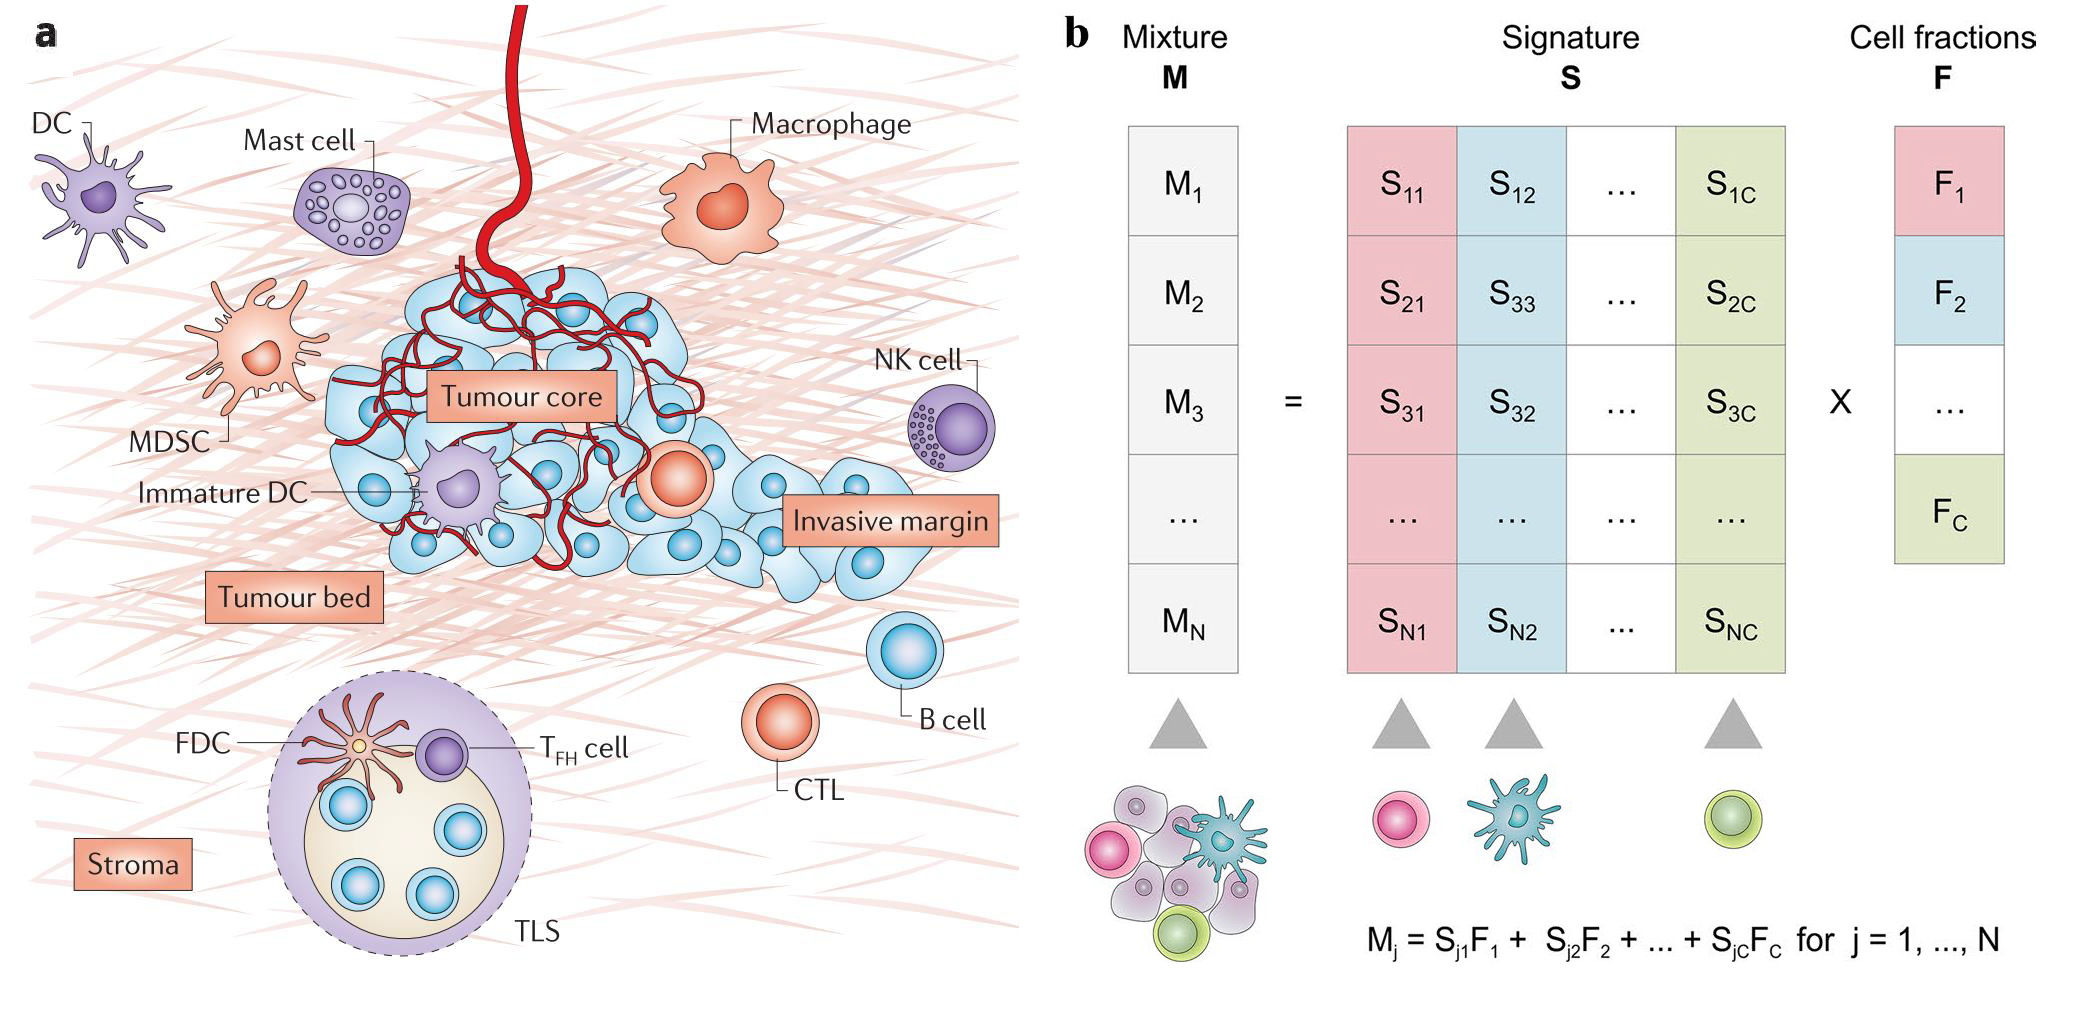
\includegraphics[width=0.8\linewidth]{images/introduction} 

}

\caption{Figure a by [@Fridman2017], Figure b by [@Finotello2018]}\label{fig:introductionFigure}
\end{figure}

Cell-type deconvolution is a computational method to calculate cell type
fraction from bulk RNA-seq data. This is done by leveraging precomputed
expression signatures that represent the transcriptional profiles of the
cell types of interest. The basic idea of cell-type deconvolution is
that the gene expression of a sample equals the weighted sum of the
contributions of different cell types. (Figure b) By extending the
number of samples from 1 to m, an equation can be given as follows:

\[ M = S \times F \] \[(𝒏×𝒎)=(𝒏×𝒌)×(𝒌×𝒎)\]

\(𝑀:\) Expression matrix of \(n\) genes in \(m\) samples.\\
\(𝑆:\) Specific gene expression values of \(𝑘\) cell types\\
\(𝐹:\) Relative cell type proportions in each sample

Therefore, the principle of cell-type deconvolution is that given \(𝑀\)
and \(𝑆\), find \(S\) to minimize the sum of square between \(S×F\) and
\(𝑀\).

\hypertarget{previous-works}{%
\subsection{Previous works}\label{previous-works}}

Presently, there exists a package
\href{https://icbi-lab.github.io/immunedeconv/}{immunedeconv} built by
the group of Gregor Sturm. It combines several first-generation
deconvolution tools which use fixed, internal signature matrices that
cover only a limited set of human cells. Nowadays, second-generation
tools have been developed that allow deriving cell-type-specific
expression signatures from single-cell RNA-seq (scRNA-seq). This enables
the deconvolution of any cell type profiled with single-cell
technologies. Therefore, these tools can extend their applicability to
other cell phenotypes, tissues, diseases, and organisms.

Our interface unifies multiple second-generation deconvolution methods
to facilitate the usage of these tools and clear the way for future
benchmarking of these methods.

\hypertarget{usage-of-immunedeconv2}{%
\section{2. Usage of Immunedeconv2}\label{usage-of-immunedeconv2}}

In this section, we want to present our package immunedeconv2 by first
giving an overview about the basic functions and the showing an example
workflow.

\hypertarget{installation-and-setup}{%
\subsection{Installation and Setup}\label{installation-and-setup}}

Install the CRAN package devtools and use it to install immunedeconv2
from \href{https://github.com/}{GitHub}:

\begin{Shaded}
\begin{Highlighting}[]
\FunctionTok{install.packages}\NormalTok{(}\StringTok{"devtools"}\NormalTok{)}
\NormalTok{devtools}\SpecialCharTok{::}\FunctionTok{install\_github}\NormalTok{(}\StringTok{"icbi{-}lab/immunedeconv2"}\NormalTok{)}
\end{Highlighting}
\end{Shaded}

\hypertarget{input-data}{%
\subsection{Input Data}\label{input-data}}

First of all, you need some data to run the deconvolution with.

\begin{itemize}
\tightlist
\item
  Single cell RNA-seq data

  \begin{itemize}
  \tightlist
  \item
    \emph{Genes} x \emph{Cells} matrix
  \item
    Counts are \emph{not log-transformed}
  \item
    Rownames (gene names) are provided in the same format as in the bulk
    RNA-seq data, for instance HGNC symbols
  \end{itemize}
\item
  Cell type annotations

  \begin{itemize}
  \tightlist
  \item
    Vector containing cell type annotations
  \item
    Annotations are in the same order as the columns of the single cell
    matrix
  \end{itemize}
\item
  Bulk RNA-seq data

  \begin{itemize}
  \tightlist
  \item
    \emph{Genes} x \emph{Samples} matrix
  \item
    Rownames (gene names) are provided in the same format as in the sc
    RNA-seq data, for instance HGNC symbols
  \end{itemize}
\end{itemize}

We also provide some sample data, a bigger and a smaller set of single
cell RNA-seq matrix (subset of
(\protect\hyperlink{ref-Maynard2020}{Maynard 2020})), cell type
annotations and bulk RNA-seq matrix
(\protect\hyperlink{ref-Hoek2015}{Hoek 2015}). You can simply load it
with:

\begin{Shaded}
\begin{Highlighting}[]
\FunctionTok{data}\NormalTok{(}\StringTok{"single\_cell\_data"}\NormalTok{)}
\FunctionTok{data}\NormalTok{(}\StringTok{"cell\_type\_annotations"}\NormalTok{)}
\FunctionTok{data}\NormalTok{(}\StringTok{"bulk"}\NormalTok{)}
\end{Highlighting}
\end{Shaded}

For the small dataset, append "\_small" to the names, e.g.~

\begin{Shaded}
\begin{Highlighting}[]
\FunctionTok{data}\NormalTok{(}\StringTok{"single\_cell\_data\_small"}\NormalTok{)}
\end{Highlighting}
\end{Shaded}

\hypertarget{signature-matrix}{%
\subsection{Signature Matrix}\label{signature-matrix}}

To calculate a cell-type-specific expression signature, you can use the
build\_model function with the single cell RNA-seq matrix and cell type
annotations specified above. The parameter method can be set to one of
the five methods listed below. More information of the methods is
provided in section 3.

\begin{Shaded}
\begin{Highlighting}[]
\NormalTok{immunedeconv2}\SpecialCharTok{::}\FunctionTok{build\_model}\NormalTok{(single\_cell\_data, cell\_type\_annotations, }
\NormalTok{    method)}
\end{Highlighting}
\end{Shaded}

\begin{itemize}
\tightlist
\item
  Bisque (``bisque'')
\item
  DWLS (``dwls'')
\item
  MOMF (``momf'')
\item
  Scaden (``scaden'')
\item
  CibersortX (``cibersortx'')
\end{itemize}

Note: MOMF and Scaden also require the bulk RNA-seq data to calculate a
signature matrix. Please provide this parameter as well when running
build\_model with one of these two methods.

Additional parameters for the different methods can be included in the
method call as well. For further information on which options you have,
see the documentation of each tool.

\hypertarget{deconvolution-of-bulk-rna-seq-data}{%
\subsection{Deconvolution of Bulk RNA-seq
Data}\label{deconvolution-of-bulk-rna-seq-data}}

After building the specific signature matrix, you can calculate the cell
properties in bulk RNA-seq data with the deconvolute function. For this,
you need to provide the bulk data, signature matrix and you can, again,
choose between the five methods listed in the previous section.

\begin{Shaded}
\begin{Highlighting}[]
\NormalTok{immunedeconv2}\SpecialCharTok{::}\FunctionTok{deconvolute}\NormalTok{(bulk, signature\_matrix, method)}
\end{Highlighting}
\end{Shaded}

Note: Bisque and MOMF additionally need the single cell RNA-seq matrix
you used to build the signature matrix for their deconvolution. As a
fifth parameter, Bisque also needs cell type annotations, which were
already needed for building the model.

Similar to the build\_model function, specific parameters can be passed
on to the deconvolution methods through the deconvolute function.

\hypertarget{example-workflow}{%
\subsection{Example Workflow}\label{example-workflow}}

This workflow provides a more detailed example of how to run the
deconvolution with Bisque.

First of all, make sure you load all the libraries we need for this
analysis. If the packages are not available, install them via
install\_packages().

\begin{Shaded}
\begin{Highlighting}[]
\FunctionTok{library}\NormalTok{(tidyr)}
\FunctionTok{library}\NormalTok{(dplyr)}
\FunctionTok{library}\NormalTok{(immunedeconv2)}
\FunctionTok{library}\NormalTok{(RColorBrewer)}
\FunctionTok{library}\NormalTok{(ggplot2)}
\end{Highlighting}
\end{Shaded}

To give you a feeling for the data, this is what a few rows and columns
of our small single cell RNA-seq dataset look like. This specific
selection of rows and columns was performed as the first rows and
columns just show zeros. Do not be alarmed by a great number of zeros in
your single cell data, this is normal:

\begin{Shaded}
\begin{Highlighting}[]
\NormalTok{knitr}\SpecialCharTok{::}\FunctionTok{kable}\NormalTok{(single\_cell\_data[}\DecValTok{170}\SpecialCharTok{:}\DecValTok{175}\NormalTok{, }\DecValTok{9}\SpecialCharTok{:}\DecValTok{13}\NormalTok{])}
\end{Highlighting}
\end{Shaded}

\begin{longtable}[]{@{}lrrrrr@{}}
\toprule
& SRR10786616 & SRR10784434 & SRR10789525 & SRR10784492 &
SRR10797498\tabularnewline
\midrule
\endhead
CXCL2 & 0.0000 & 6853.19729 & 1085.391633 & 5568.45845 &
1716.1670\tabularnewline
IMPG2 & 0.0000 & 0.00000 & 0.000000 & 0.00000 & 0.0000\tabularnewline
PTPRC & 549.8070 & 19.17636 & 34.114055 & 13.37534 &
131.8831\tabularnewline
STK17B & 281.3871 & 0.00000 & 6.824202 & 0.00000 &
132.8119\tabularnewline
PCDHA6 & 0.0000 & 0.00000 & 0.000000 & 0.00000 & 0.0000\tabularnewline
IL12RB2 & 0.0000 & 0.00000 & 0.000000 & 0.00000 & 0.0000\tabularnewline
\bottomrule
\end{longtable}

Now we build the signature matrix with Bisque and look at the values for
the first few genes.

\begin{Shaded}
\begin{Highlighting}[]
\NormalTok{signatureMatrix }\OtherTok{\textless{}{-}}\NormalTok{ immunedeconv2}\SpecialCharTok{::}\FunctionTok{build\_model}\NormalTok{(single\_cell\_data, }
\NormalTok{    cell\_type\_annotations, }\StringTok{"bisque"}\NormalTok{)}
\NormalTok{knitr}\SpecialCharTok{::}\FunctionTok{kable}\NormalTok{(signatureMatrix[}\DecValTok{1}\SpecialCharTok{:}\DecValTok{5}\NormalTok{, ])}
\end{Highlighting}
\end{Shaded}

\begin{longtable}[]{@{}lrrrrrrrrr@{}}
\toprule
\begin{minipage}[b]{(\columnwidth - 9\tabcolsep) * \real{0.06}}\raggedright
\strut
\end{minipage} &
\begin{minipage}[b]{(\columnwidth - 9\tabcolsep) * \real{0.06}}\raggedleft
B cell\strut
\end{minipage} &
\begin{minipage}[b]{(\columnwidth - 9\tabcolsep) * \real{0.08}}\raggedleft
Macrophage\strut
\end{minipage} &
\begin{minipage}[b]{(\columnwidth - 9\tabcolsep) * \real{0.16}}\raggedleft
Monocyte conventional\strut
\end{minipage} &
\begin{minipage}[b]{(\columnwidth - 9\tabcolsep) * \real{0.18}}\raggedleft
Monocyte non-conventional\strut
\end{minipage} &
\begin{minipage}[b]{(\columnwidth - 9\tabcolsep) * \real{0.06}}\raggedleft
NK cell\strut
\end{minipage} &
\begin{minipage}[b]{(\columnwidth - 9\tabcolsep) * \real{0.08}}\raggedleft
T cell CD4\strut
\end{minipage} &
\begin{minipage}[b]{(\columnwidth - 9\tabcolsep) * \real{0.08}}\raggedleft
T cell CD8\strut
\end{minipage} &
\begin{minipage}[b]{(\columnwidth - 9\tabcolsep) * \real{0.11}}\raggedleft
T cell dividing\strut
\end{minipage} &
\begin{minipage}[b]{(\columnwidth - 9\tabcolsep) * \real{0.13}}\raggedleft
T cell regulatory\strut
\end{minipage}\tabularnewline
\midrule
\endhead
\begin{minipage}[t]{(\columnwidth - 9\tabcolsep) * \real{0.06}}\raggedright
TSPAN6\strut
\end{minipage} &
\begin{minipage}[t]{(\columnwidth - 9\tabcolsep) * \real{0.06}}\raggedleft
0.00000\strut
\end{minipage} &
\begin{minipage}[t]{(\columnwidth - 9\tabcolsep) * \real{0.08}}\raggedleft
0.0224404\strut
\end{minipage} &
\begin{minipage}[t]{(\columnwidth - 9\tabcolsep) * \real{0.16}}\raggedleft
0.00000\strut
\end{minipage} &
\begin{minipage}[t]{(\columnwidth - 9\tabcolsep) * \real{0.18}}\raggedleft
0.000000\strut
\end{minipage} &
\begin{minipage}[t]{(\columnwidth - 9\tabcolsep) * \real{0.06}}\raggedleft
0.00000\strut
\end{minipage} &
\begin{minipage}[t]{(\columnwidth - 9\tabcolsep) * \real{0.08}}\raggedleft
0.0000000\strut
\end{minipage} &
\begin{minipage}[t]{(\columnwidth - 9\tabcolsep) * \real{0.08}}\raggedleft
0.0000000\strut
\end{minipage} &
\begin{minipage}[t]{(\columnwidth - 9\tabcolsep) * \real{0.11}}\raggedleft
0.000000\strut
\end{minipage} &
\begin{minipage}[t]{(\columnwidth - 9\tabcolsep) * \real{0.13}}\raggedleft
0.0000\strut
\end{minipage}\tabularnewline
\begin{minipage}[t]{(\columnwidth - 9\tabcolsep) * \real{0.06}}\raggedright
FGR\strut
\end{minipage} &
\begin{minipage}[t]{(\columnwidth - 9\tabcolsep) * \real{0.06}}\raggedleft
14.43455\strut
\end{minipage} &
\begin{minipage}[t]{(\columnwidth - 9\tabcolsep) * \real{0.08}}\raggedleft
30.7676144\strut
\end{minipage} &
\begin{minipage}[t]{(\columnwidth - 9\tabcolsep) * \real{0.16}}\raggedleft
313.40391\strut
\end{minipage} &
\begin{minipage}[t]{(\columnwidth - 9\tabcolsep) * \real{0.18}}\raggedleft
180.407874\strut
\end{minipage} &
\begin{minipage}[t]{(\columnwidth - 9\tabcolsep) * \real{0.06}}\raggedleft
77.97797\strut
\end{minipage} &
\begin{minipage}[t]{(\columnwidth - 9\tabcolsep) * \real{0.08}}\raggedleft
0.1278529\strut
\end{minipage} &
\begin{minipage}[t]{(\columnwidth - 9\tabcolsep) * \real{0.08}}\raggedleft
0.7800284\strut
\end{minipage} &
\begin{minipage}[t]{(\columnwidth - 9\tabcolsep) * \real{0.11}}\raggedleft
0.000000\strut
\end{minipage} &
\begin{minipage}[t]{(\columnwidth - 9\tabcolsep) * \real{0.13}}\raggedleft
0.0000\strut
\end{minipage}\tabularnewline
\begin{minipage}[t]{(\columnwidth - 9\tabcolsep) * \real{0.06}}\raggedright
CYP51A1\strut
\end{minipage} &
\begin{minipage}[t]{(\columnwidth - 9\tabcolsep) * \real{0.06}}\raggedleft
30.79303\strut
\end{minipage} &
\begin{minipage}[t]{(\columnwidth - 9\tabcolsep) * \real{0.08}}\raggedleft
10.9460034\strut
\end{minipage} &
\begin{minipage}[t]{(\columnwidth - 9\tabcolsep) * \real{0.16}}\raggedleft
13.19608\strut
\end{minipage} &
\begin{minipage}[t]{(\columnwidth - 9\tabcolsep) * \real{0.18}}\raggedleft
5.456035\strut
\end{minipage} &
\begin{minipage}[t]{(\columnwidth - 9\tabcolsep) * \real{0.06}}\raggedleft
22.90308\strut
\end{minipage} &
\begin{minipage}[t]{(\columnwidth - 9\tabcolsep) * \real{0.08}}\raggedleft
11.1332235\strut
\end{minipage} &
\begin{minipage}[t]{(\columnwidth - 9\tabcolsep) * \real{0.08}}\raggedleft
20.7037599\strut
\end{minipage} &
\begin{minipage}[t]{(\columnwidth - 9\tabcolsep) * \real{0.11}}\raggedleft
9.325876\strut
\end{minipage} &
\begin{minipage}[t]{(\columnwidth - 9\tabcolsep) * \real{0.13}}\raggedleft
20.4159\strut
\end{minipage}\tabularnewline
\begin{minipage}[t]{(\columnwidth - 9\tabcolsep) * \real{0.06}}\raggedright
AOC1\strut
\end{minipage} &
\begin{minipage}[t]{(\columnwidth - 9\tabcolsep) * \real{0.06}}\raggedleft
0.00000\strut
\end{minipage} &
\begin{minipage}[t]{(\columnwidth - 9\tabcolsep) * \real{0.08}}\raggedleft
0.0900427\strut
\end{minipage} &
\begin{minipage}[t]{(\columnwidth - 9\tabcolsep) * \real{0.16}}\raggedleft
0.00000\strut
\end{minipage} &
\begin{minipage}[t]{(\columnwidth - 9\tabcolsep) * \real{0.18}}\raggedleft
8.219547\strut
\end{minipage} &
\begin{minipage}[t]{(\columnwidth - 9\tabcolsep) * \real{0.06}}\raggedleft
0.00000\strut
\end{minipage} &
\begin{minipage}[t]{(\columnwidth - 9\tabcolsep) * \real{0.08}}\raggedleft
0.0000000\strut
\end{minipage} &
\begin{minipage}[t]{(\columnwidth - 9\tabcolsep) * \real{0.08}}\raggedleft
0.0000000\strut
\end{minipage} &
\begin{minipage}[t]{(\columnwidth - 9\tabcolsep) * \real{0.11}}\raggedleft
0.000000\strut
\end{minipage} &
\begin{minipage}[t]{(\columnwidth - 9\tabcolsep) * \real{0.13}}\raggedleft
0.0000\strut
\end{minipage}\tabularnewline
\begin{minipage}[t]{(\columnwidth - 9\tabcolsep) * \real{0.06}}\raggedright
WNT16\strut
\end{minipage} &
\begin{minipage}[t]{(\columnwidth - 9\tabcolsep) * \real{0.06}}\raggedleft
11.65795\strut
\end{minipage} &
\begin{minipage}[t]{(\columnwidth - 9\tabcolsep) * \real{0.08}}\raggedleft
0.0309828\strut
\end{minipage} &
\begin{minipage}[t]{(\columnwidth - 9\tabcolsep) * \real{0.16}}\raggedleft
0.00000\strut
\end{minipage} &
\begin{minipage}[t]{(\columnwidth - 9\tabcolsep) * \real{0.18}}\raggedleft
0.000000\strut
\end{minipage} &
\begin{minipage}[t]{(\columnwidth - 9\tabcolsep) * \real{0.06}}\raggedleft
0.00000\strut
\end{minipage} &
\begin{minipage}[t]{(\columnwidth - 9\tabcolsep) * \real{0.08}}\raggedleft
0.0000000\strut
\end{minipage} &
\begin{minipage}[t]{(\columnwidth - 9\tabcolsep) * \real{0.08}}\raggedleft
0.0000000\strut
\end{minipage} &
\begin{minipage}[t]{(\columnwidth - 9\tabcolsep) * \real{0.11}}\raggedleft
0.000000\strut
\end{minipage} &
\begin{minipage}[t]{(\columnwidth - 9\tabcolsep) * \real{0.13}}\raggedleft
0.0000\strut
\end{minipage}\tabularnewline
\bottomrule
\end{longtable}

We can use this signature matrix to run the deconvolution with Bisque.

\begin{Shaded}
\begin{Highlighting}[]
\NormalTok{immunedeconv2}\SpecialCharTok{::}\FunctionTok{deconvolute}\NormalTok{(bulk, signatureMatrix, }\StringTok{"bisque"}\NormalTok{, single\_cell\_data, }
\NormalTok{    cell\_type\_annotations) }\SpecialCharTok{\%\textgreater{}\%}\NormalTok{ knitr}\SpecialCharTok{::}\FunctionTok{kable}\NormalTok{()}
\end{Highlighting}
\end{Shaded}

\begin{longtable}[]{@{}lrrrrrrrrr@{}}
\toprule
\begin{minipage}[b]{(\columnwidth - 9\tabcolsep) * \real{0.08}}\raggedright
\strut
\end{minipage} &
\begin{minipage}[b]{(\columnwidth - 9\tabcolsep) * \real{0.07}}\raggedleft
B cell\strut
\end{minipage} &
\begin{minipage}[b]{(\columnwidth - 9\tabcolsep) * \real{0.07}}\raggedleft
Macrophage\strut
\end{minipage} &
\begin{minipage}[b]{(\columnwidth - 9\tabcolsep) * \real{0.15}}\raggedleft
Monocyte conventional\strut
\end{minipage} &
\begin{minipage}[b]{(\columnwidth - 9\tabcolsep) * \real{0.18}}\raggedleft
Monocyte non conventional\strut
\end{minipage} &
\begin{minipage}[b]{(\columnwidth - 9\tabcolsep) * \real{0.07}}\raggedleft
NK cell\strut
\end{minipage} &
\begin{minipage}[b]{(\columnwidth - 9\tabcolsep) * \real{0.07}}\raggedleft
T cell CD4\strut
\end{minipage} &
\begin{minipage}[b]{(\columnwidth - 9\tabcolsep) * \real{0.07}}\raggedleft
T cell CD8\strut
\end{minipage} &
\begin{minipage}[b]{(\columnwidth - 9\tabcolsep) * \real{0.11}}\raggedleft
T cell dividing\strut
\end{minipage} &
\begin{minipage}[b]{(\columnwidth - 9\tabcolsep) * \real{0.12}}\raggedleft
T cell regulatory\strut
\end{minipage}\tabularnewline
\midrule
\endhead
\begin{minipage}[t]{(\columnwidth - 9\tabcolsep) * \real{0.08}}\raggedright
HD30\_PBMC\_0\strut
\end{minipage} &
\begin{minipage}[t]{(\columnwidth - 9\tabcolsep) * \real{0.07}}\raggedleft
0.0000000\strut
\end{minipage} &
\begin{minipage}[t]{(\columnwidth - 9\tabcolsep) * \real{0.07}}\raggedleft
0.3538763\strut
\end{minipage} &
\begin{minipage}[t]{(\columnwidth - 9\tabcolsep) * \real{0.15}}\raggedleft
0.0000000\strut
\end{minipage} &
\begin{minipage}[t]{(\columnwidth - 9\tabcolsep) * \real{0.18}}\raggedleft
0.0000000\strut
\end{minipage} &
\begin{minipage}[t]{(\columnwidth - 9\tabcolsep) * \real{0.07}}\raggedleft
0.1740958\strut
\end{minipage} &
\begin{minipage}[t]{(\columnwidth - 9\tabcolsep) * \real{0.07}}\raggedleft
0.0000000\strut
\end{minipage} &
\begin{minipage}[t]{(\columnwidth - 9\tabcolsep) * \real{0.07}}\raggedleft
0.0506317\strut
\end{minipage} &
\begin{minipage}[t]{(\columnwidth - 9\tabcolsep) * \real{0.11}}\raggedleft
0.4213961\strut
\end{minipage} &
\begin{minipage}[t]{(\columnwidth - 9\tabcolsep) * \real{0.12}}\raggedleft
0.0000000\strut
\end{minipage}\tabularnewline
\begin{minipage}[t]{(\columnwidth - 9\tabcolsep) * \real{0.08}}\raggedright
HD30\_PBMC\_1\strut
\end{minipage} &
\begin{minipage}[t]{(\columnwidth - 9\tabcolsep) * \real{0.07}}\raggedleft
0.0000000\strut
\end{minipage} &
\begin{minipage}[t]{(\columnwidth - 9\tabcolsep) * \real{0.07}}\raggedleft
0.1136076\strut
\end{minipage} &
\begin{minipage}[t]{(\columnwidth - 9\tabcolsep) * \real{0.15}}\raggedleft
0.0000000\strut
\end{minipage} &
\begin{minipage}[t]{(\columnwidth - 9\tabcolsep) * \real{0.18}}\raggedleft
0.2588127\strut
\end{minipage} &
\begin{minipage}[t]{(\columnwidth - 9\tabcolsep) * \real{0.07}}\raggedleft
0.1689959\strut
\end{minipage} &
\begin{minipage}[t]{(\columnwidth - 9\tabcolsep) * \real{0.07}}\raggedleft
0.0000000\strut
\end{minipage} &
\begin{minipage}[t]{(\columnwidth - 9\tabcolsep) * \real{0.07}}\raggedleft
0.0000000\strut
\end{minipage} &
\begin{minipage}[t]{(\columnwidth - 9\tabcolsep) * \real{0.11}}\raggedleft
0.4585839\strut
\end{minipage} &
\begin{minipage}[t]{(\columnwidth - 9\tabcolsep) * \real{0.12}}\raggedleft
0.0000000\strut
\end{minipage}\tabularnewline
\begin{minipage}[t]{(\columnwidth - 9\tabcolsep) * \real{0.08}}\raggedright
HD30\_PBMC\_3\strut
\end{minipage} &
\begin{minipage}[t]{(\columnwidth - 9\tabcolsep) * \real{0.07}}\raggedleft
0.0000000\strut
\end{minipage} &
\begin{minipage}[t]{(\columnwidth - 9\tabcolsep) * \real{0.07}}\raggedleft
0.1483928\strut
\end{minipage} &
\begin{minipage}[t]{(\columnwidth - 9\tabcolsep) * \real{0.15}}\raggedleft
0.0000000\strut
\end{minipage} &
\begin{minipage}[t]{(\columnwidth - 9\tabcolsep) * \real{0.18}}\raggedleft
0.0000000\strut
\end{minipage} &
\begin{minipage}[t]{(\columnwidth - 9\tabcolsep) * \real{0.07}}\raggedleft
0.2431386\strut
\end{minipage} &
\begin{minipage}[t]{(\columnwidth - 9\tabcolsep) * \real{0.07}}\raggedleft
0.3459540\strut
\end{minipage} &
\begin{minipage}[t]{(\columnwidth - 9\tabcolsep) * \real{0.07}}\raggedleft
0.0000000\strut
\end{minipage} &
\begin{minipage}[t]{(\columnwidth - 9\tabcolsep) * \real{0.11}}\raggedleft
0.2625147\strut
\end{minipage} &
\begin{minipage}[t]{(\columnwidth - 9\tabcolsep) * \real{0.12}}\raggedleft
0.0000000\strut
\end{minipage}\tabularnewline
\begin{minipage}[t]{(\columnwidth - 9\tabcolsep) * \real{0.08}}\raggedright
HD30\_PBMC\_7\strut
\end{minipage} &
\begin{minipage}[t]{(\columnwidth - 9\tabcolsep) * \real{0.07}}\raggedleft
0.0000000\strut
\end{minipage} &
\begin{minipage}[t]{(\columnwidth - 9\tabcolsep) * \real{0.07}}\raggedleft
0.2308434\strut
\end{minipage} &
\begin{minipage}[t]{(\columnwidth - 9\tabcolsep) * \real{0.15}}\raggedleft
0.0000000\strut
\end{minipage} &
\begin{minipage}[t]{(\columnwidth - 9\tabcolsep) * \real{0.18}}\raggedleft
0.0000000\strut
\end{minipage} &
\begin{minipage}[t]{(\columnwidth - 9\tabcolsep) * \real{0.07}}\raggedleft
0.1853657\strut
\end{minipage} &
\begin{minipage}[t]{(\columnwidth - 9\tabcolsep) * \real{0.07}}\raggedleft
0.0000000\strut
\end{minipage} &
\begin{minipage}[t]{(\columnwidth - 9\tabcolsep) * \real{0.07}}\raggedleft
0.4179878\strut
\end{minipage} &
\begin{minipage}[t]{(\columnwidth - 9\tabcolsep) * \real{0.11}}\raggedleft
0.1658031\strut
\end{minipage} &
\begin{minipage}[t]{(\columnwidth - 9\tabcolsep) * \real{0.12}}\raggedleft
0.0000000\strut
\end{minipage}\tabularnewline
\begin{minipage}[t]{(\columnwidth - 9\tabcolsep) * \real{0.08}}\raggedright
HD31\_PBMC\_0\strut
\end{minipage} &
\begin{minipage}[t]{(\columnwidth - 9\tabcolsep) * \real{0.07}}\raggedleft
0.0000000\strut
\end{minipage} &
\begin{minipage}[t]{(\columnwidth - 9\tabcolsep) * \real{0.07}}\raggedleft
0.5108072\strut
\end{minipage} &
\begin{minipage}[t]{(\columnwidth - 9\tabcolsep) * \real{0.15}}\raggedleft
0.3647978\strut
\end{minipage} &
\begin{minipage}[t]{(\columnwidth - 9\tabcolsep) * \real{0.18}}\raggedleft
0.0000000\strut
\end{minipage} &
\begin{minipage}[t]{(\columnwidth - 9\tabcolsep) * \real{0.07}}\raggedleft
0.0000000\strut
\end{minipage} &
\begin{minipage}[t]{(\columnwidth - 9\tabcolsep) * \real{0.07}}\raggedleft
0.1243950\strut
\end{minipage} &
\begin{minipage}[t]{(\columnwidth - 9\tabcolsep) * \real{0.07}}\raggedleft
0.0000000\strut
\end{minipage} &
\begin{minipage}[t]{(\columnwidth - 9\tabcolsep) * \real{0.11}}\raggedleft
0.0000000\strut
\end{minipage} &
\begin{minipage}[t]{(\columnwidth - 9\tabcolsep) * \real{0.12}}\raggedleft
0.0000000\strut
\end{minipage}\tabularnewline
\begin{minipage}[t]{(\columnwidth - 9\tabcolsep) * \real{0.08}}\raggedright
HD31\_PBMC\_1\strut
\end{minipage} &
\begin{minipage}[t]{(\columnwidth - 9\tabcolsep) * \real{0.07}}\raggedleft
0.0000000\strut
\end{minipage} &
\begin{minipage}[t]{(\columnwidth - 9\tabcolsep) * \real{0.07}}\raggedleft
0.3681902\strut
\end{minipage} &
\begin{minipage}[t]{(\columnwidth - 9\tabcolsep) * \real{0.15}}\raggedleft
0.1929607\strut
\end{minipage} &
\begin{minipage}[t]{(\columnwidth - 9\tabcolsep) * \real{0.18}}\raggedleft
0.2083132\strut
\end{minipage} &
\begin{minipage}[t]{(\columnwidth - 9\tabcolsep) * \real{0.07}}\raggedleft
0.0000000\strut
\end{minipage} &
\begin{minipage}[t]{(\columnwidth - 9\tabcolsep) * \real{0.07}}\raggedleft
0.2305358\strut
\end{minipage} &
\begin{minipage}[t]{(\columnwidth - 9\tabcolsep) * \real{0.07}}\raggedleft
0.0000000\strut
\end{minipage} &
\begin{minipage}[t]{(\columnwidth - 9\tabcolsep) * \real{0.11}}\raggedleft
0.0000000\strut
\end{minipage} &
\begin{minipage}[t]{(\columnwidth - 9\tabcolsep) * \real{0.12}}\raggedleft
0.0000000\strut
\end{minipage}\tabularnewline
\begin{minipage}[t]{(\columnwidth - 9\tabcolsep) * \real{0.08}}\raggedright
HD31\_PBMC\_3\strut
\end{minipage} &
\begin{minipage}[t]{(\columnwidth - 9\tabcolsep) * \real{0.07}}\raggedleft
0.1603286\strut
\end{minipage} &
\begin{minipage}[t]{(\columnwidth - 9\tabcolsep) * \real{0.07}}\raggedleft
0.1429087\strut
\end{minipage} &
\begin{minipage}[t]{(\columnwidth - 9\tabcolsep) * \real{0.15}}\raggedleft
0.2630120\strut
\end{minipage} &
\begin{minipage}[t]{(\columnwidth - 9\tabcolsep) * \real{0.18}}\raggedleft
0.0000000\strut
\end{minipage} &
\begin{minipage}[t]{(\columnwidth - 9\tabcolsep) * \real{0.07}}\raggedleft
0.0000000\strut
\end{minipage} &
\begin{minipage}[t]{(\columnwidth - 9\tabcolsep) * \real{0.07}}\raggedleft
0.2268409\strut
\end{minipage} &
\begin{minipage}[t]{(\columnwidth - 9\tabcolsep) * \real{0.07}}\raggedleft
0.0000000\strut
\end{minipage} &
\begin{minipage}[t]{(\columnwidth - 9\tabcolsep) * \real{0.11}}\raggedleft
0.0000000\strut
\end{minipage} &
\begin{minipage}[t]{(\columnwidth - 9\tabcolsep) * \real{0.12}}\raggedleft
0.2069098\strut
\end{minipage}\tabularnewline
\begin{minipage}[t]{(\columnwidth - 9\tabcolsep) * \real{0.08}}\raggedright
HD31\_PBMC\_7\strut
\end{minipage} &
\begin{minipage}[t]{(\columnwidth - 9\tabcolsep) * \real{0.07}}\raggedleft
0.0000000\strut
\end{minipage} &
\begin{minipage}[t]{(\columnwidth - 9\tabcolsep) * \real{0.07}}\raggedleft
0.4834342\strut
\end{minipage} &
\begin{minipage}[t]{(\columnwidth - 9\tabcolsep) * \real{0.15}}\raggedleft
0.1360895\strut
\end{minipage} &
\begin{minipage}[t]{(\columnwidth - 9\tabcolsep) * \real{0.18}}\raggedleft
0.0000000\strut
\end{minipage} &
\begin{minipage}[t]{(\columnwidth - 9\tabcolsep) * \real{0.07}}\raggedleft
0.0000000\strut
\end{minipage} &
\begin{minipage}[t]{(\columnwidth - 9\tabcolsep) * \real{0.07}}\raggedleft
0.0711957\strut
\end{minipage} &
\begin{minipage}[t]{(\columnwidth - 9\tabcolsep) * \real{0.07}}\raggedleft
0.0000000\strut
\end{minipage} &
\begin{minipage}[t]{(\columnwidth - 9\tabcolsep) * \real{0.11}}\raggedleft
0.0000000\strut
\end{minipage} &
\begin{minipage}[t]{(\columnwidth - 9\tabcolsep) * \real{0.12}}\raggedleft
0.3092806\strut
\end{minipage}\tabularnewline
\bottomrule
\end{longtable}

\hypertarget{plot-results}{%
\subsection{Plot Results}\label{plot-results}}

Additionally, we provide some methods for visualisation. In this and the
benchmarking section you can find examples of how to use them. For the
plotDeconvResult method, you can additionally provide a method and file
name to add a title to your plot and save it.

\begin{Shaded}
\begin{Highlighting}[]
\NormalTok{res\_bisque }\OtherTok{\textless{}{-}}\NormalTok{ immunedeconv2}\SpecialCharTok{::}\FunctionTok{deconvolute}\NormalTok{(bulk, signatureMatrix, }
    \StringTok{"bisque"}\NormalTok{, single\_cell\_data, cell\_type\_annotations)}
\NormalTok{immunedeconv2}\SpecialCharTok{::}\FunctionTok{plotDeconvResult}\NormalTok{(res\_bisque, }\AttributeTok{method =} \StringTok{"Bisque"}\NormalTok{)}
\end{Highlighting}
\end{Shaded}

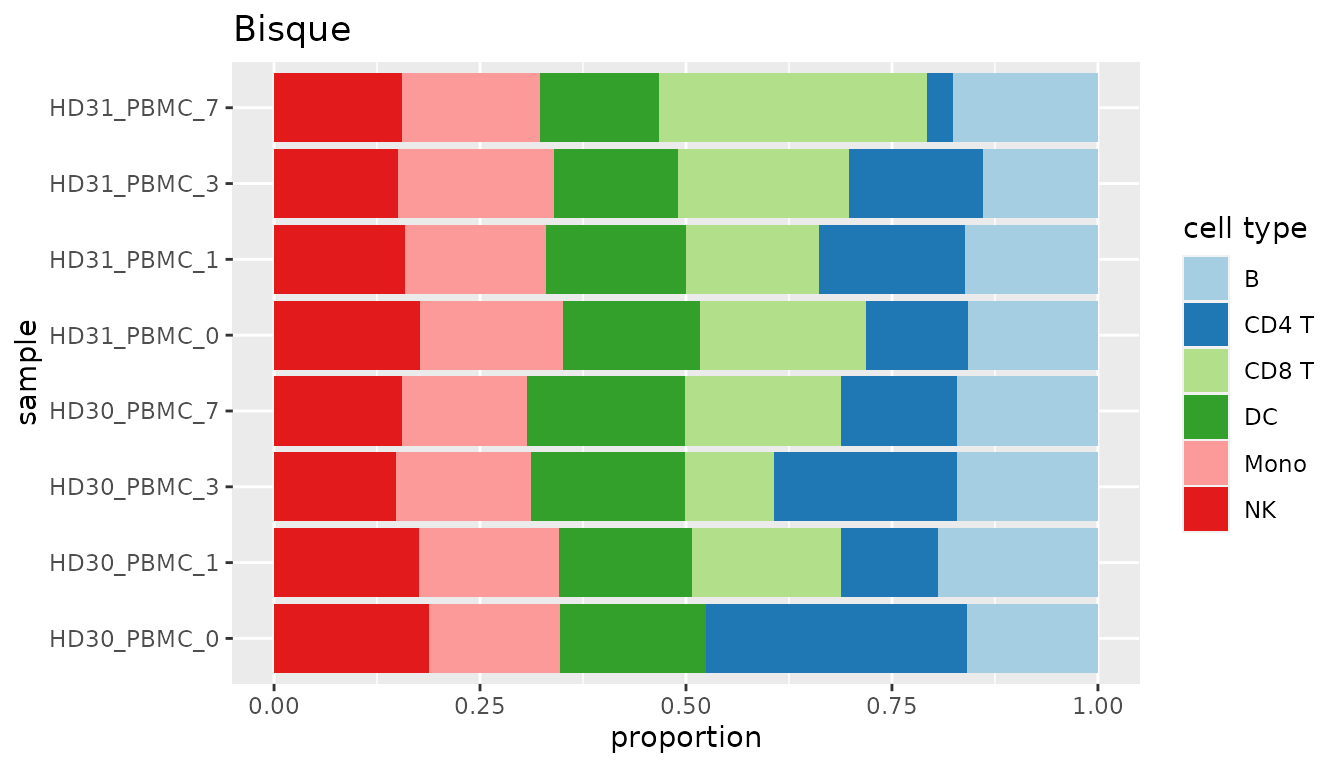
\includegraphics{immunedeconv2_vignette_files/figure-latex/plot-1.pdf}

The scatterplot shown below depicts the same results and message as the
barplot above, it is just another idea of how to visualize the results.
Note that our package does not provide a method for this, but the plot
can be recreated with this code.

\begin{Shaded}
\begin{Highlighting}[]
\FunctionTok{data.frame}\NormalTok{(res\_bisque, }\AttributeTok{samples =} \FunctionTok{rownames}\NormalTok{(res\_bisque)) }\SpecialCharTok{\%\textgreater{}\%} \FunctionTok{pivot\_longer}\NormalTok{(}\SpecialCharTok{!}\NormalTok{samples, }
    \AttributeTok{names\_to =} \StringTok{"cell\_type"}\NormalTok{, }\AttributeTok{values\_to =} \StringTok{"predicted\_fraction"}\NormalTok{) }\SpecialCharTok{\%\textgreater{}\%} 
    \FunctionTok{ggplot}\NormalTok{(}\FunctionTok{aes}\NormalTok{(}\AttributeTok{y =}\NormalTok{ samples, }\AttributeTok{x =}\NormalTok{ predicted\_fraction, }\AttributeTok{color =}\NormalTok{ cell\_type)) }\SpecialCharTok{+} 
    \FunctionTok{geom\_point}\NormalTok{(}\AttributeTok{size =} \DecValTok{3}\NormalTok{) }\SpecialCharTok{+} \FunctionTok{facet\_wrap}\NormalTok{(}\SpecialCharTok{\textasciitilde{}}\NormalTok{cell\_type) }\SpecialCharTok{+} \FunctionTok{labs}\NormalTok{(}\AttributeTok{title =} \StringTok{"Bisque"}\NormalTok{, }
    \AttributeTok{y =} \StringTok{"sample"}\NormalTok{, }\AttributeTok{x =} \StringTok{"predicted fraction"}\NormalTok{, }\AttributeTok{color =} \StringTok{"cell type"}\NormalTok{) }\SpecialCharTok{+} 
    \FunctionTok{scale\_fill\_brewer}\NormalTok{(}\AttributeTok{palette =} \StringTok{"Paired"}\NormalTok{)}
\end{Highlighting}
\end{Shaded}

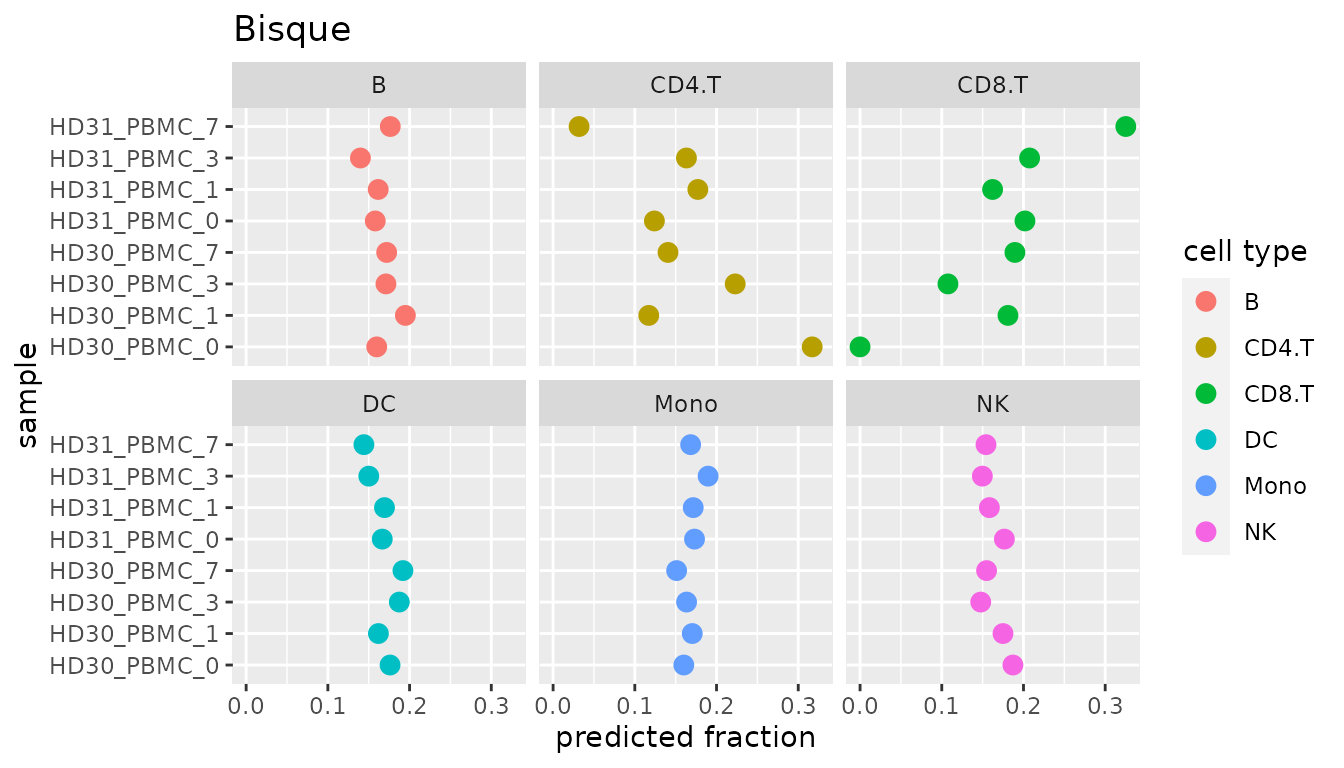
\includegraphics{immunedeconv2_vignette_files/figure-latex/plot2-1.pdf}

In the next figures you can see how the other methods are used and how
the cell proportions would be distributed based on their calculations.
Here are some further ideas of how you could plot your deconvolution
results.

\begin{Shaded}
\begin{Highlighting}[]
\NormalTok{res\_momf }\OtherTok{\textless{}{-}}\NormalTok{ immunedeconv2}\SpecialCharTok{::}\FunctionTok{build\_model}\NormalTok{(single\_cell\_data, cell\_type\_annotations, }
    \StringTok{"momf"}\NormalTok{, bulk) }\SpecialCharTok{\%\textgreater{}\%}\NormalTok{ immunedeconv2}\SpecialCharTok{::}\FunctionTok{deconvolute}\NormalTok{(}\AttributeTok{bulk\_gene\_expression =}\NormalTok{ bulk, }
    \AttributeTok{method =} \StringTok{"momf"}\NormalTok{, }\AttributeTok{single\_cell\_object =}\NormalTok{ single\_cell\_data)}
\NormalTok{immunedeconv2}\SpecialCharTok{::}\FunctionTok{plotDeconvResult}\NormalTok{(res\_momf, }\AttributeTok{method =} \StringTok{"MOMF"}\NormalTok{)}
\NormalTok{res\_scaden }\OtherTok{\textless{}{-}}\NormalTok{ immunedeconv2}\SpecialCharTok{::}\FunctionTok{build\_model}\NormalTok{(}\AttributeTok{single\_cell\_object =}\NormalTok{ single\_cell\_data, }
    \AttributeTok{cell\_type\_annotations =}\NormalTok{ cell\_type\_annotations, }\AttributeTok{method =} \StringTok{"scaden"}\NormalTok{, }
\NormalTok{    bulk) }\SpecialCharTok{\%\textgreater{}\%}\NormalTok{ immunedeconv2}\SpecialCharTok{::}\FunctionTok{deconvolute}\NormalTok{(}\AttributeTok{bulk\_gene\_expression =}\NormalTok{ bulk, }
    \AttributeTok{method =} \StringTok{"scaden"}\NormalTok{, }\AttributeTok{single\_cell\_object =}\NormalTok{ single\_cell\_data)}
\NormalTok{immunedeconv2}\SpecialCharTok{::}\FunctionTok{plotDeconvResult}\NormalTok{(res\_scaden, }\AttributeTok{method =} \StringTok{"Scaden"}\NormalTok{)}
\NormalTok{res\_dwls }\OtherTok{\textless{}{-}}\NormalTok{ immunedeconv2}\SpecialCharTok{::}\FunctionTok{build\_model}\NormalTok{(single\_cell\_data, cell\_type\_annotations, }
    \StringTok{"dwls"}\NormalTok{) }\SpecialCharTok{\%\textgreater{}\%}\NormalTok{ immunedeconv2}\SpecialCharTok{::}\FunctionTok{deconvolute}\NormalTok{(}\AttributeTok{bulk\_gene\_expression =}\NormalTok{ bulk, }
    \AttributeTok{method =} \StringTok{"dwls"}\NormalTok{)}
\NormalTok{immunedeconv2}\SpecialCharTok{::}\FunctionTok{plotDeconvResult}\NormalTok{(res\_dwls, }\AttributeTok{method =} \StringTok{"DWLS"}\NormalTok{)}
\NormalTok{res\_ciber }\OtherTok{\textless{}{-}}\NormalTok{ immunedeconv2}\SpecialCharTok{::}\FunctionTok{build\_model}\NormalTok{(single\_cell\_data, cell\_type\_annotations, }
    \StringTok{"cibersortx"}\NormalTok{) }\SpecialCharTok{\%\textgreater{}\%}\NormalTok{ immunedeconv2}\SpecialCharTok{::}\FunctionTok{deconvolute}\NormalTok{(}\AttributeTok{bulk\_gene\_expression =}\NormalTok{ bulk, }
    \AttributeTok{method =} \StringTok{"cibersortx"}\NormalTok{)}
\NormalTok{immunedeconv2}\SpecialCharTok{::}\FunctionTok{plotDeconvResult}\NormalTok{(res\_ciber, }\AttributeTok{method =} \StringTok{"CibersortX"}\NormalTok{)}
\end{Highlighting}
\end{Shaded}

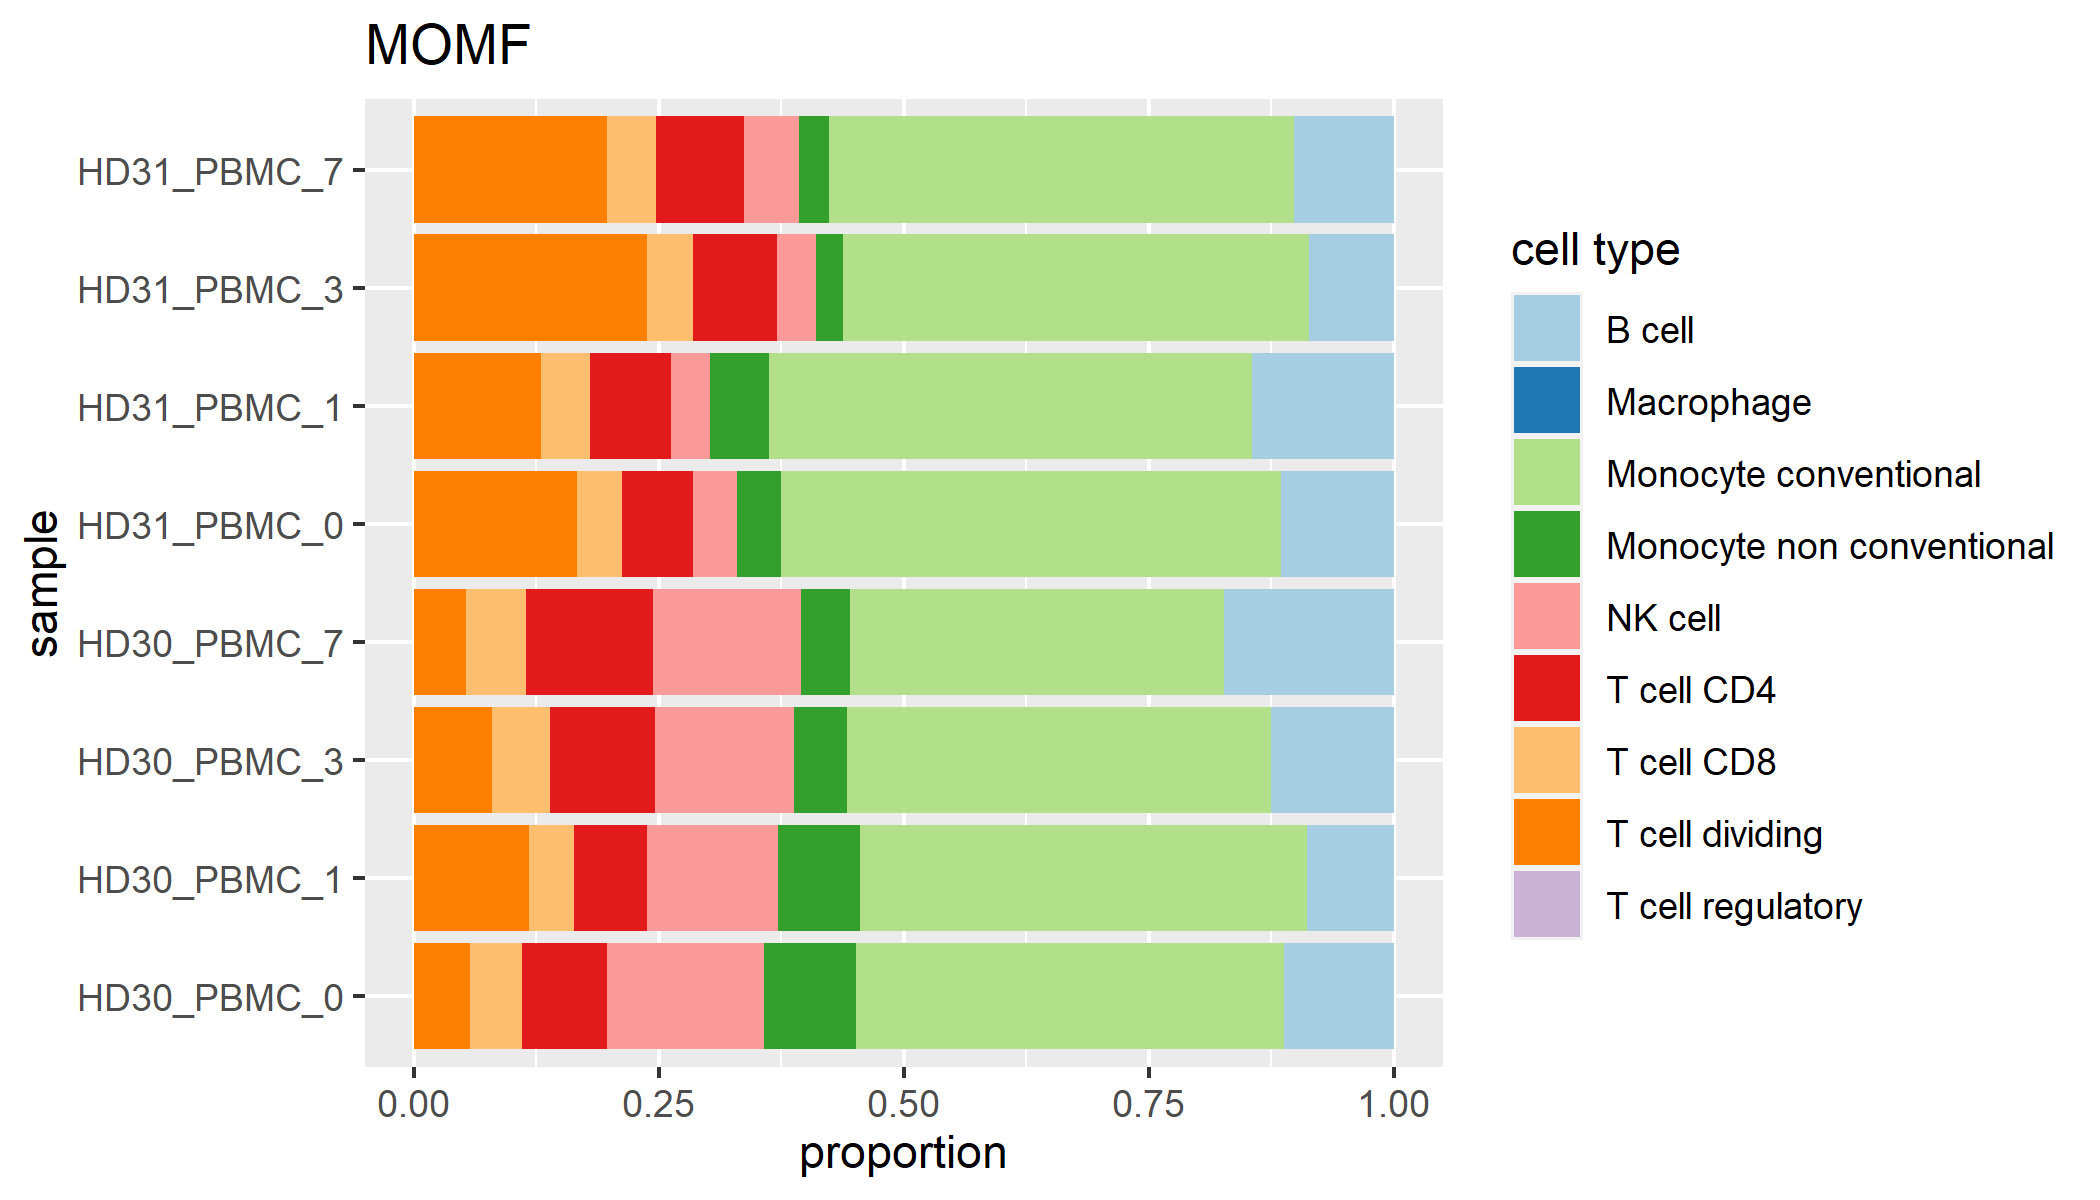
\includegraphics[width=0.8\linewidth]{images/momf_prop}
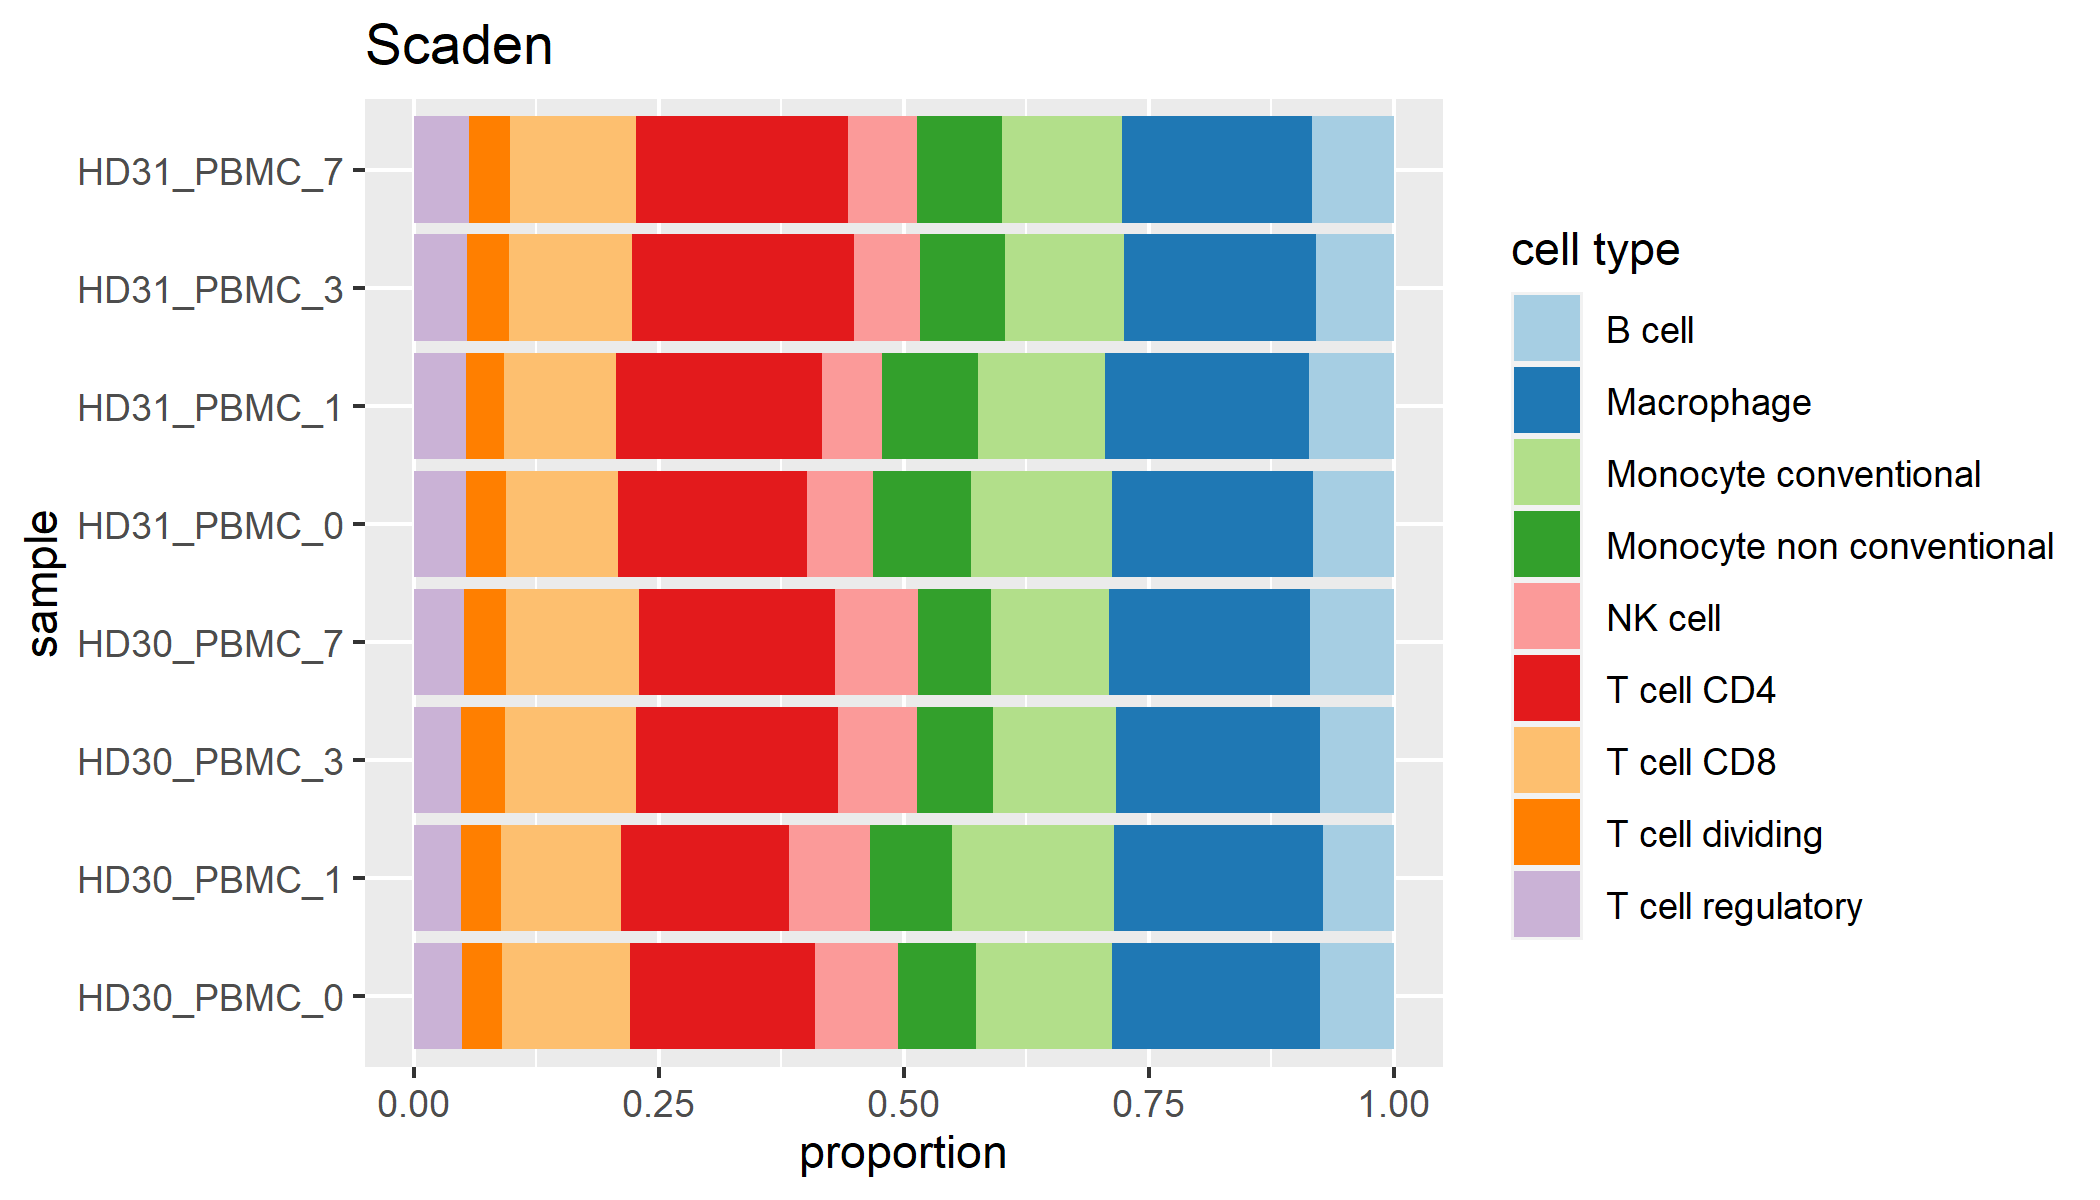
\includegraphics[width=0.8\linewidth]{images/scaden_prop}
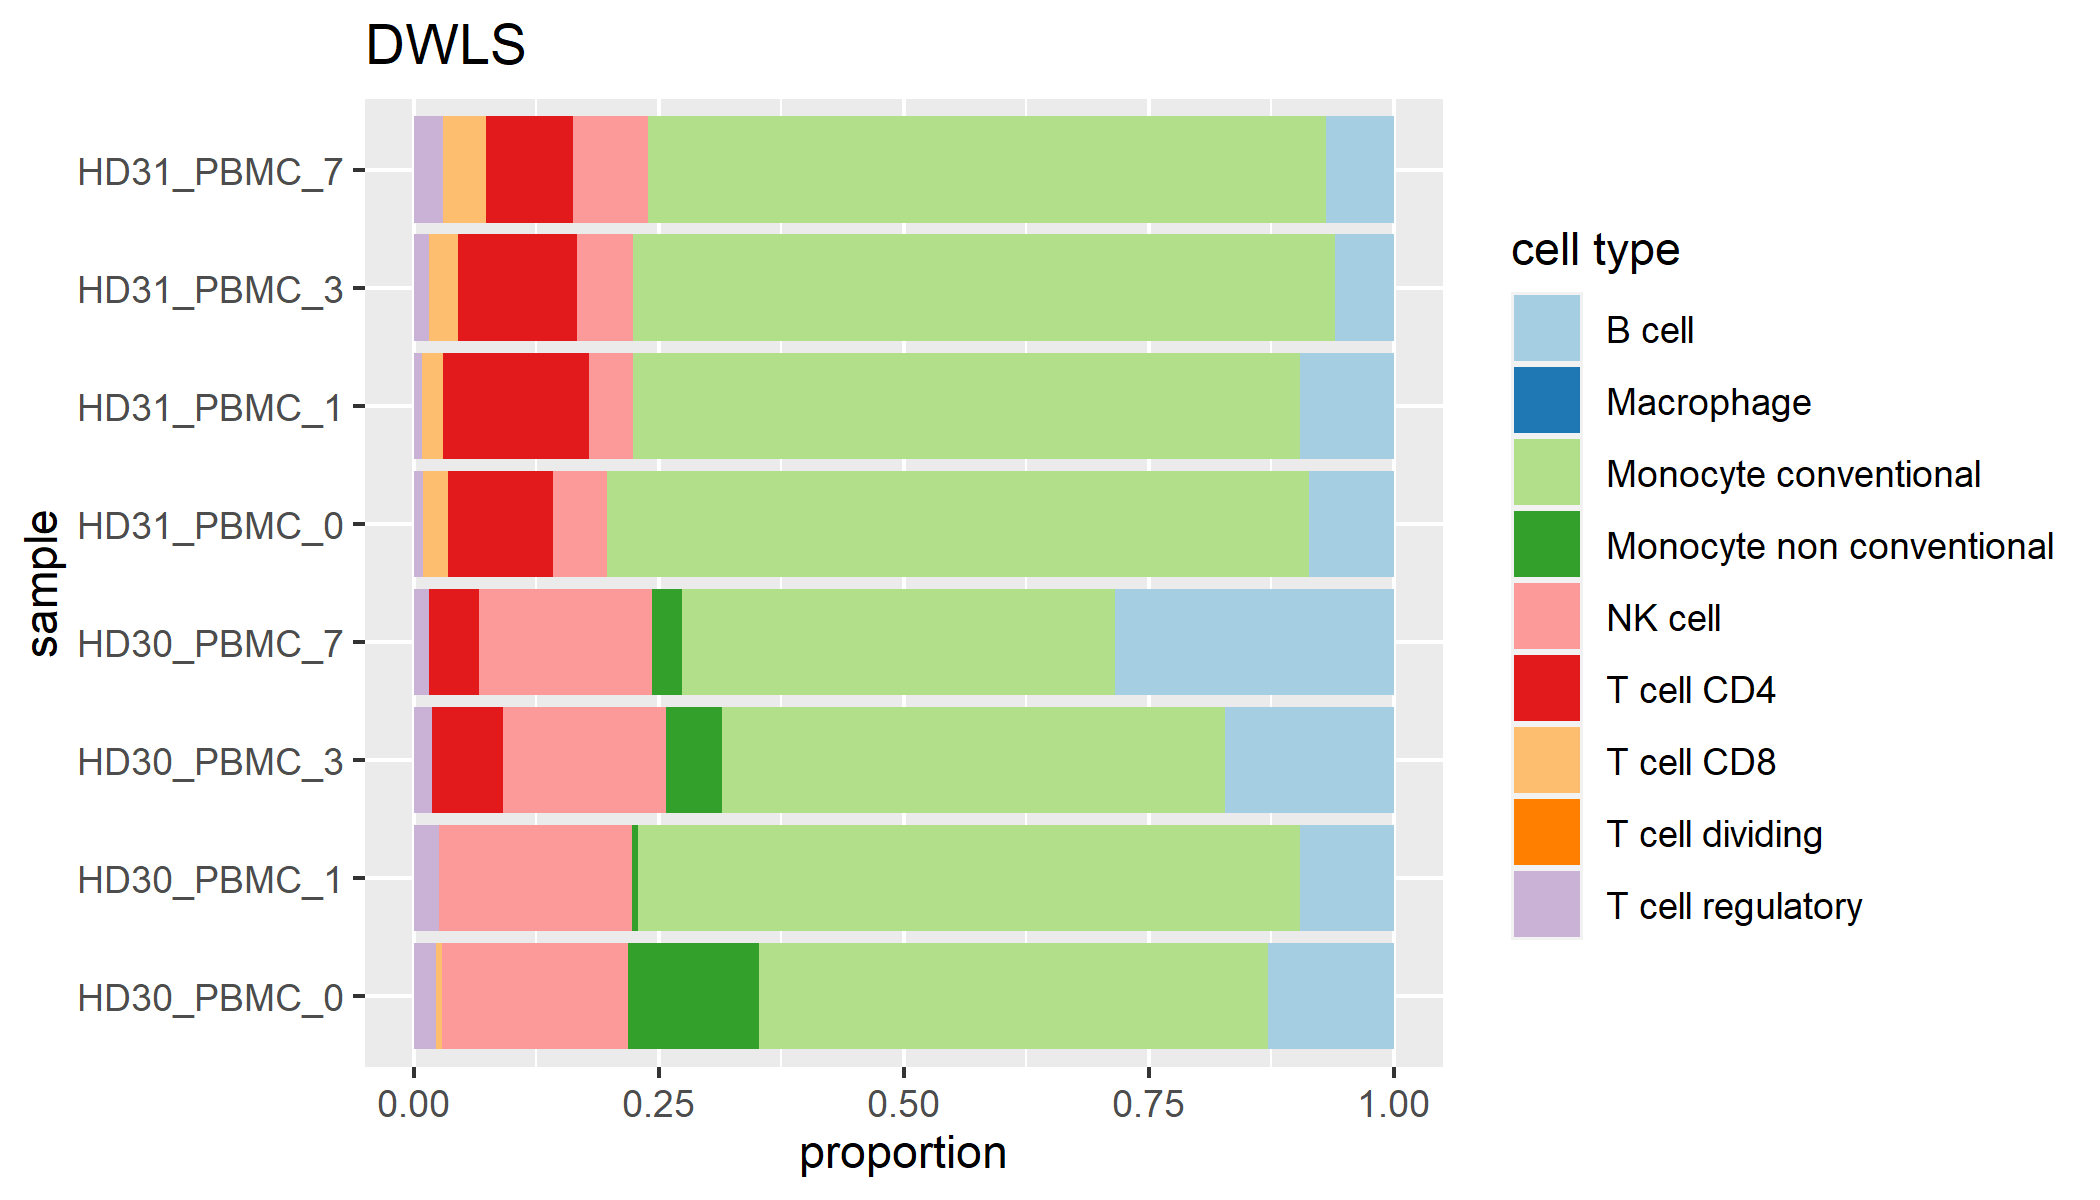
\includegraphics[width=0.8\linewidth]{images/dwls_prop}
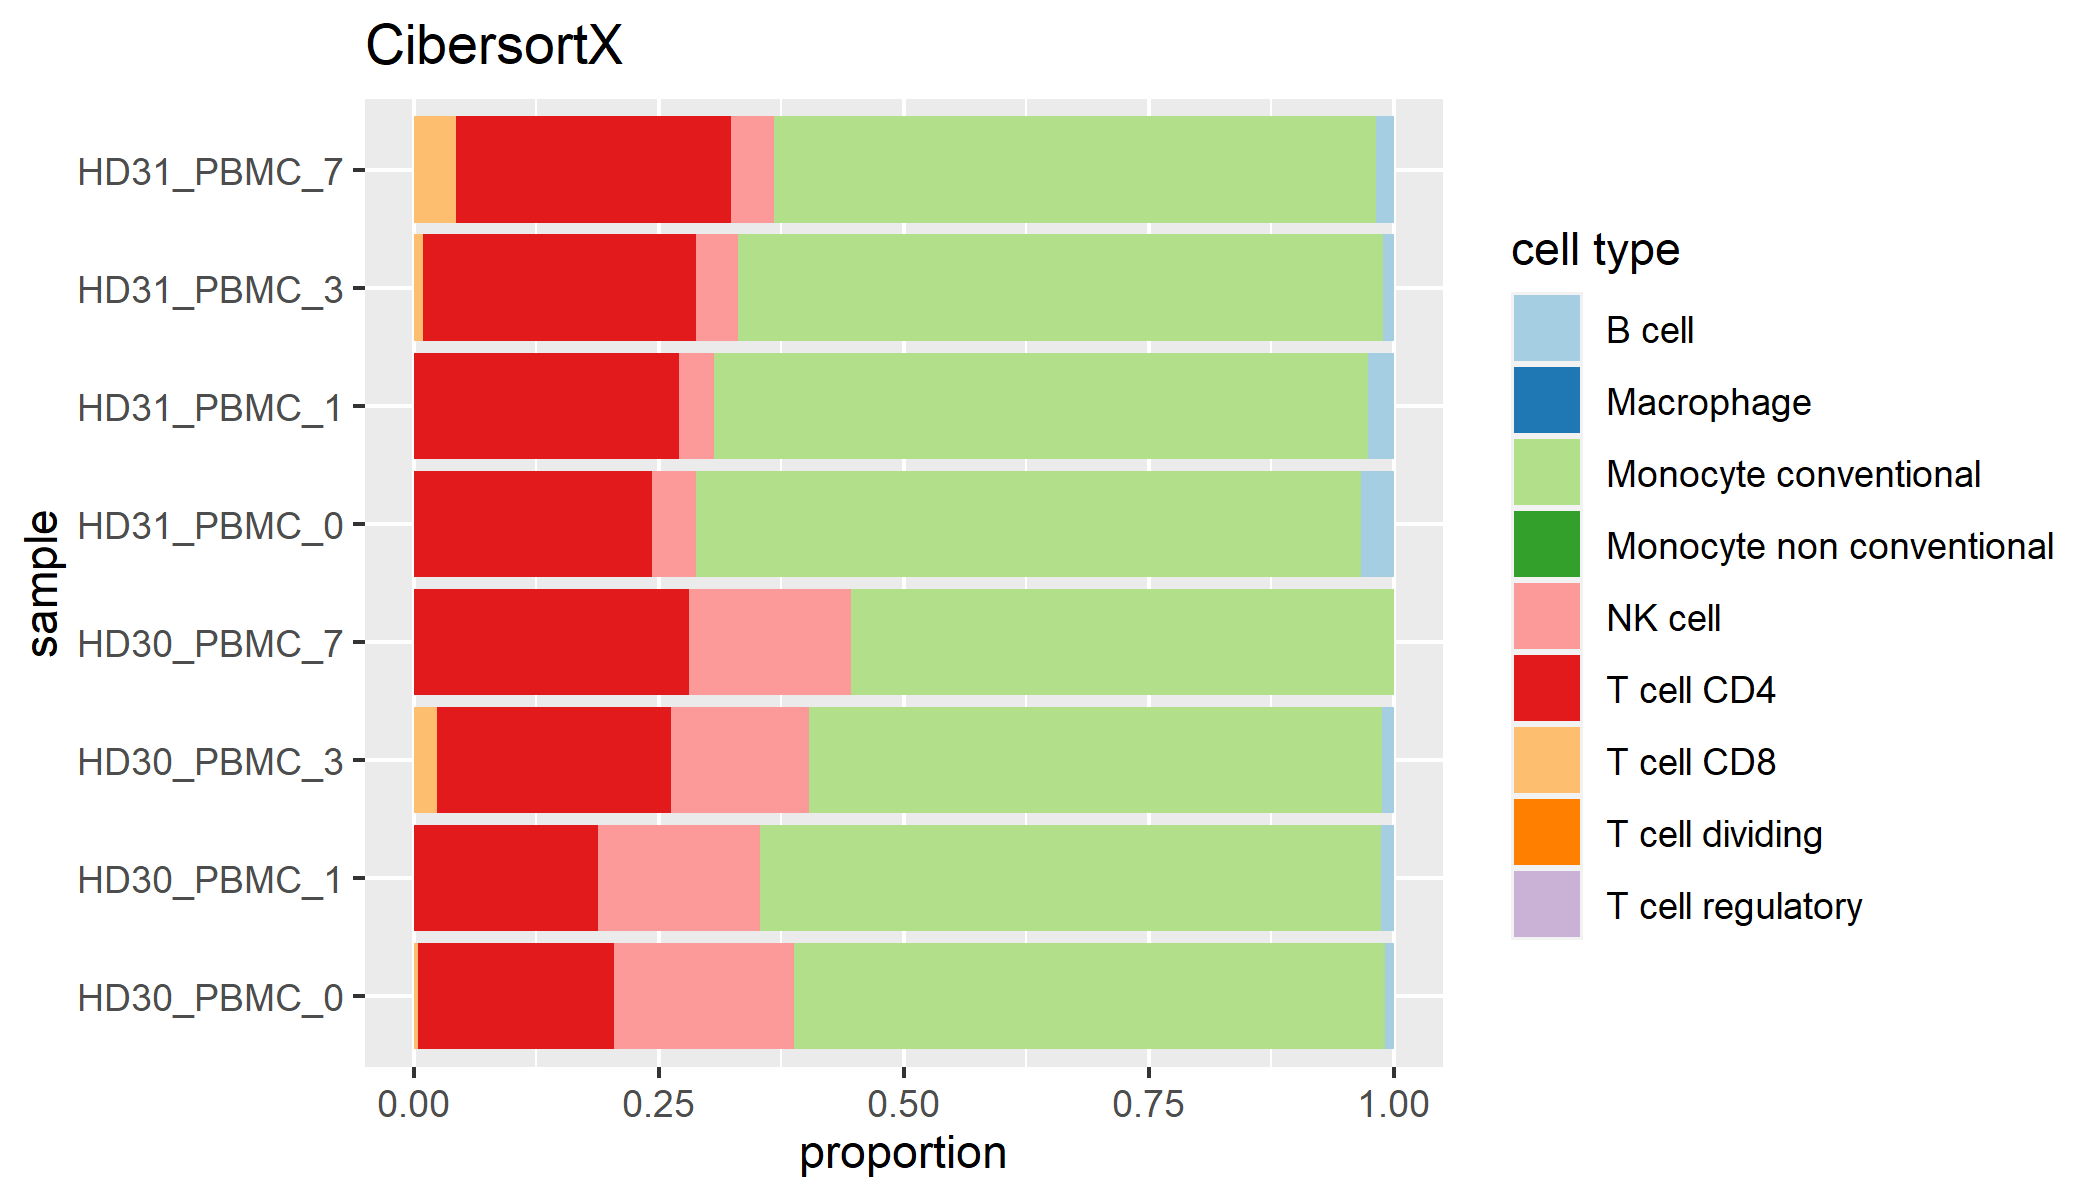
\includegraphics[width=0.8\linewidth]{images/cibersortx_prop}

\hypertarget{methods}{%
\section{3. Methods}\label{methods}}

In this section, we provide a short overview over the deconvolution
methods that can be used via this package.

Please note that even though our package is freely available, the second
generation immune deconvolution methods may not be. For instance, the
usage of CibersortX requires a token bound to your IP address. For more
information and to request such a token, please see the official website
\href{https://cibersortx.stanford.edu/}{CIBERSORTX}.

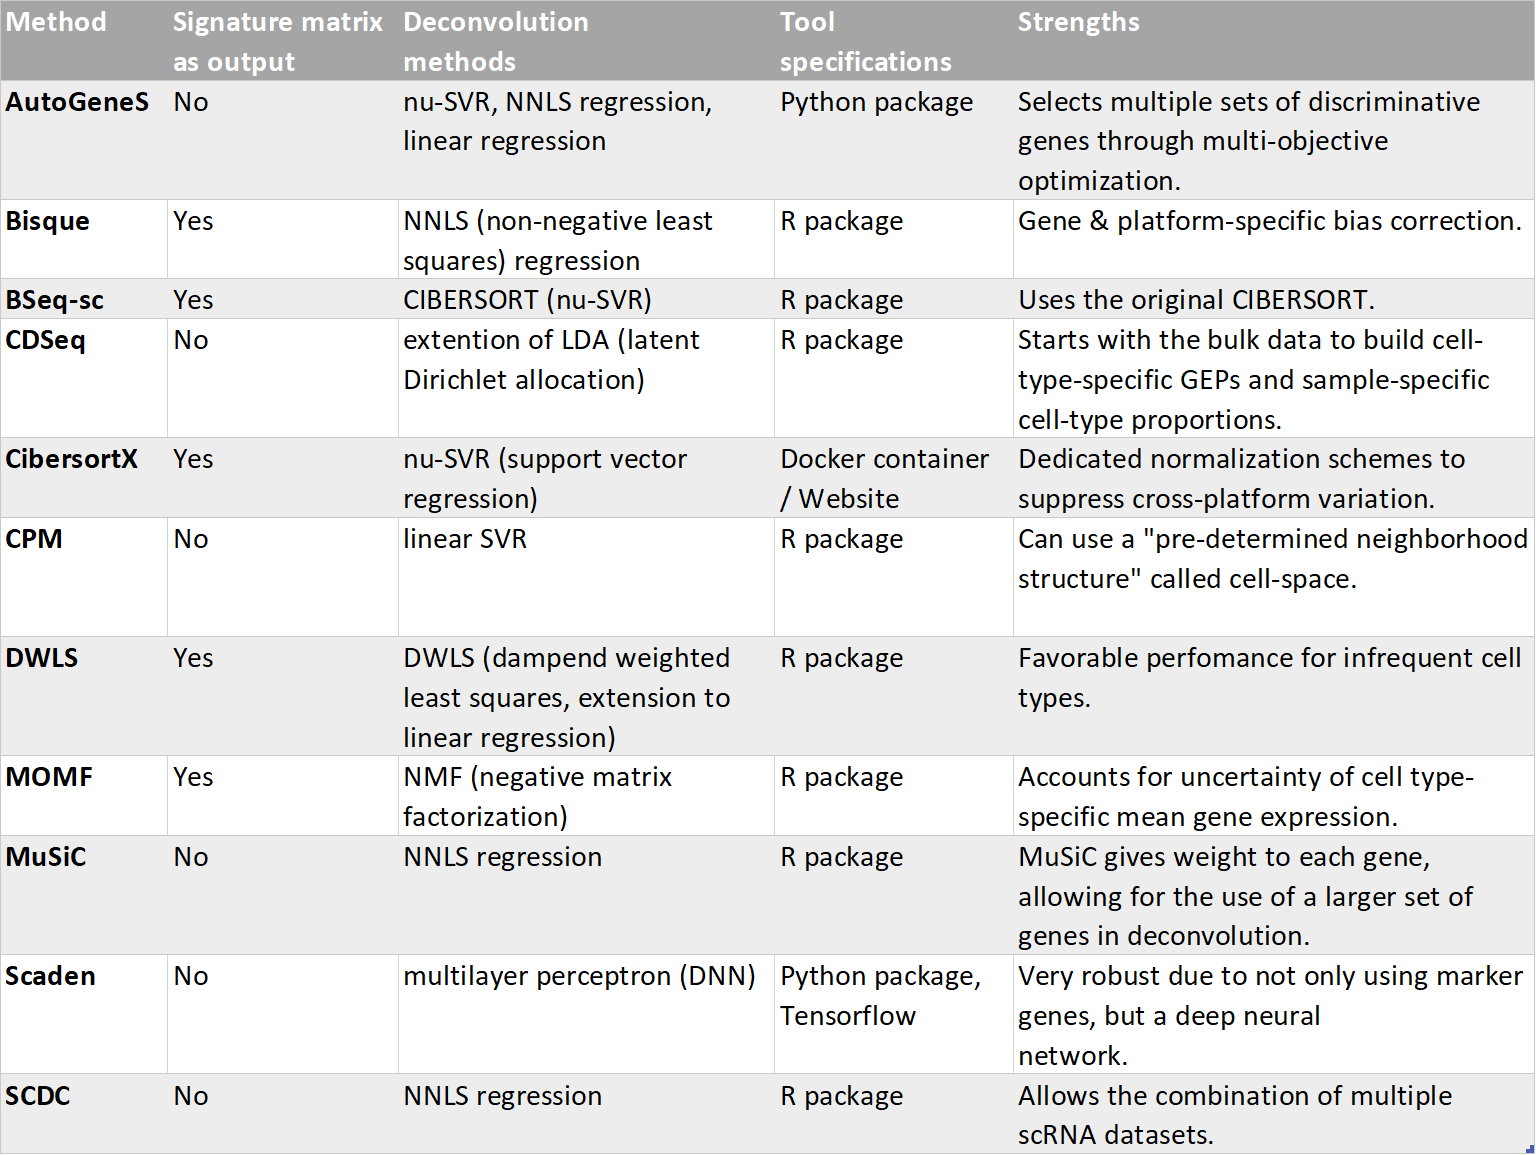
\includegraphics[width=0.8\linewidth]{images/methods_table}

\hypertarget{bisque}{%
\subsection{Bisque}\label{bisque}}

Bisque takes advantage of matched bulk and scRNA-seq samples to improve
accuracy of cell-type estimates. Using linear regression, it corrects
for platform-specific biases between pseudo-bulk reference profiles
derived from scRNA-seq and bulk RNA-seq samples. It then applies
NNLS-regression to deconvolute other bulk RNA-seq samples.

Citation: Jew, B., Alvarez, M., Rahmani, E., Miao, Z., Ko, A., Garske,
K. M., Sul, J. H., Pietiläinen, K. H., Pajukanta, P., \& Halperin, E.
(2020). Publisher Correction: Accurate estimation of cell composition in
bulk expression through robust integration of single-cell information.
Nature Communications, 11(1), 2891.
\url{https://doi.org/10.1038/s41467-020-16607-9}

\hypertarget{cibersortx}{%
\subsection{CibersortX}\label{cibersortx}}

CIBERSORTx is an extension to the original CIBERSORT algorithm
(\protect\hyperlink{ref-Newman2015}{Newman 2015}) that enables building
signature matrices from scRNA-seq or sorted bulk RNA-seq samples based
on differential gene expression analysis. To address technical biases
they introduce two batch correction methods, one designed to mitigate
batch effects between datasets, the other to address differences between
sequencing protocols (e.g.~10x vs.~full-length). Moreover, CIBERSORTx
supports ``complete'' deconvolution, not only yielding cell-type
proportions but disentangling bulk gene expression profiles into
cell-type specific expression profiles.

Citation: Newman, A. M., Liu, C. L., Green, M. R., Gentles, A. J., Feng,
W., Xu, Y., Hoang, C. D., Diehn, M., \& Alizadeh, A. A. (2015). Robust
enumeration of cell subsets from tissue expression profiles. Nature
Methods, 12(5), 453--457. \url{https://doi.org/10.1038/nmeth.3337}

\hypertarget{dwls}{%
\subsection{DWLS}\label{dwls}}

Tsoucas et al.~introduce dampened weighted least squares
(DWLS)-regression, which improves over ordinary least squares regression
or 𝜈-SVR in that it attributes higher weight to rare cell types and
marker genes with a low average expression level. They show that their
method achieves favorable performance when estimating the abundance of
infrequent cell-types.

Citation: Tsoucas, D., Dong, R., Chen, H., Zhu, Q., Guo, G., \& Yuan,
G.-C. (2019). Accurate estimation of cell-type composition from gene
expression data. Nature Communications, 10(1), 2975.
\url{https://doi.org/10.1038/s41467-019-10802-z}

\hypertarget{momf}{%
\subsection{MOMF}\label{momf}}

With MOMF, Multi-Omics Matrix Factorization, models the cell type
specific mean in scRNA-seq data by also accounting for the uncertainty
of these cell type specific mean gene expression levels. Alternating
Direction Method of Multipliers algorithm is then used to estimate the
parameters in bulk RNA-seq downstream analyses.

Citation: Xifang Sun, Shiquan Sun, and Sheng Yang. An efficient and
flexible method for deconvoluting bulk RNAseq data with single-cell
RNAseq data, 2019, DIO: 10.5281/zenodo.3373980

\hypertarget{scaden}{%
\subsection{Scaden}\label{scaden}}

Scaden leverages a deep neural network (DNN) for estimating cell-type
proportions. Instead of explicitly building a signature matrix, the DNN
implicitly learns which features are important for a certain cell type.
The DNN is trained by simulating bulk RNA-seq samples with known
cell-type proportions from scRNA-seq datasets. To increase robustness,
the training process allows to flexibly integrate multiple scRNA-seq
datasets and, optionally, bulk RNA-seq samples with ``gold standard''
measurements such as FACS.

Citation: Menden, K., Marouf, M., Oller, S., Dalmia, A., Kloiber, K.,
Heutink, P., \& Bonn, S. (n.d.). Deep-learning-based cell composition
analysis from tissue expression profiles.
\url{https://doi.org/10.1101/659227}

\hypertarget{benchmarking}{%
\section{4. Benchmarking}\label{benchmarking}}

To evaluate the performance of the methods used, we compared a data set
with 17k cells (\protect\hyperlink{ref-Hoek2015}{Hoek 2015}) to its
ground truth, measured with FACS. This data is also included in our
benchmarking method, which takes the desired filename and -type as a
parameter, as a testset.

For this comparison, a perfect estimation of cell type fractions by one
method would include that all points align to the diagonal line in the
according facet.

\hypertarget{prediction-results}{%
\subsection{Prediction results}\label{prediction-results}}

In the two figures shown below, both bulk and single cell RNA-seq data
are TPM normalized. This is the standard for this kind of data and our
test data sets contain TPM normalized values as well.

\begin{Shaded}
\begin{Highlighting}[]
\NormalTok{result\_list }\OtherTok{\textless{}{-}} \FunctionTok{c}\NormalTok{(}\AttributeTok{Bisque =}\NormalTok{ res\_bisque, }\AttributeTok{CibersortX =}\NormalTok{ res\_ciber, }
    \AttributeTok{DWLS =}\NormalTok{ res\_dwls, }\AttributeTok{MOMF =}\NormalTok{ res\_momf, }\AttributeTok{Scaden =}\NormalTok{ res\_scaden)}
\NormalTok{immunedeconv2}\SpecialCharTok{::}\FunctionTok{makeBenchmarkingScatterplot}\NormalTok{(result\_list, }\StringTok{"predictionVsGroundtruth.png"}\NormalTok{)}
\end{Highlighting}
\end{Shaded}

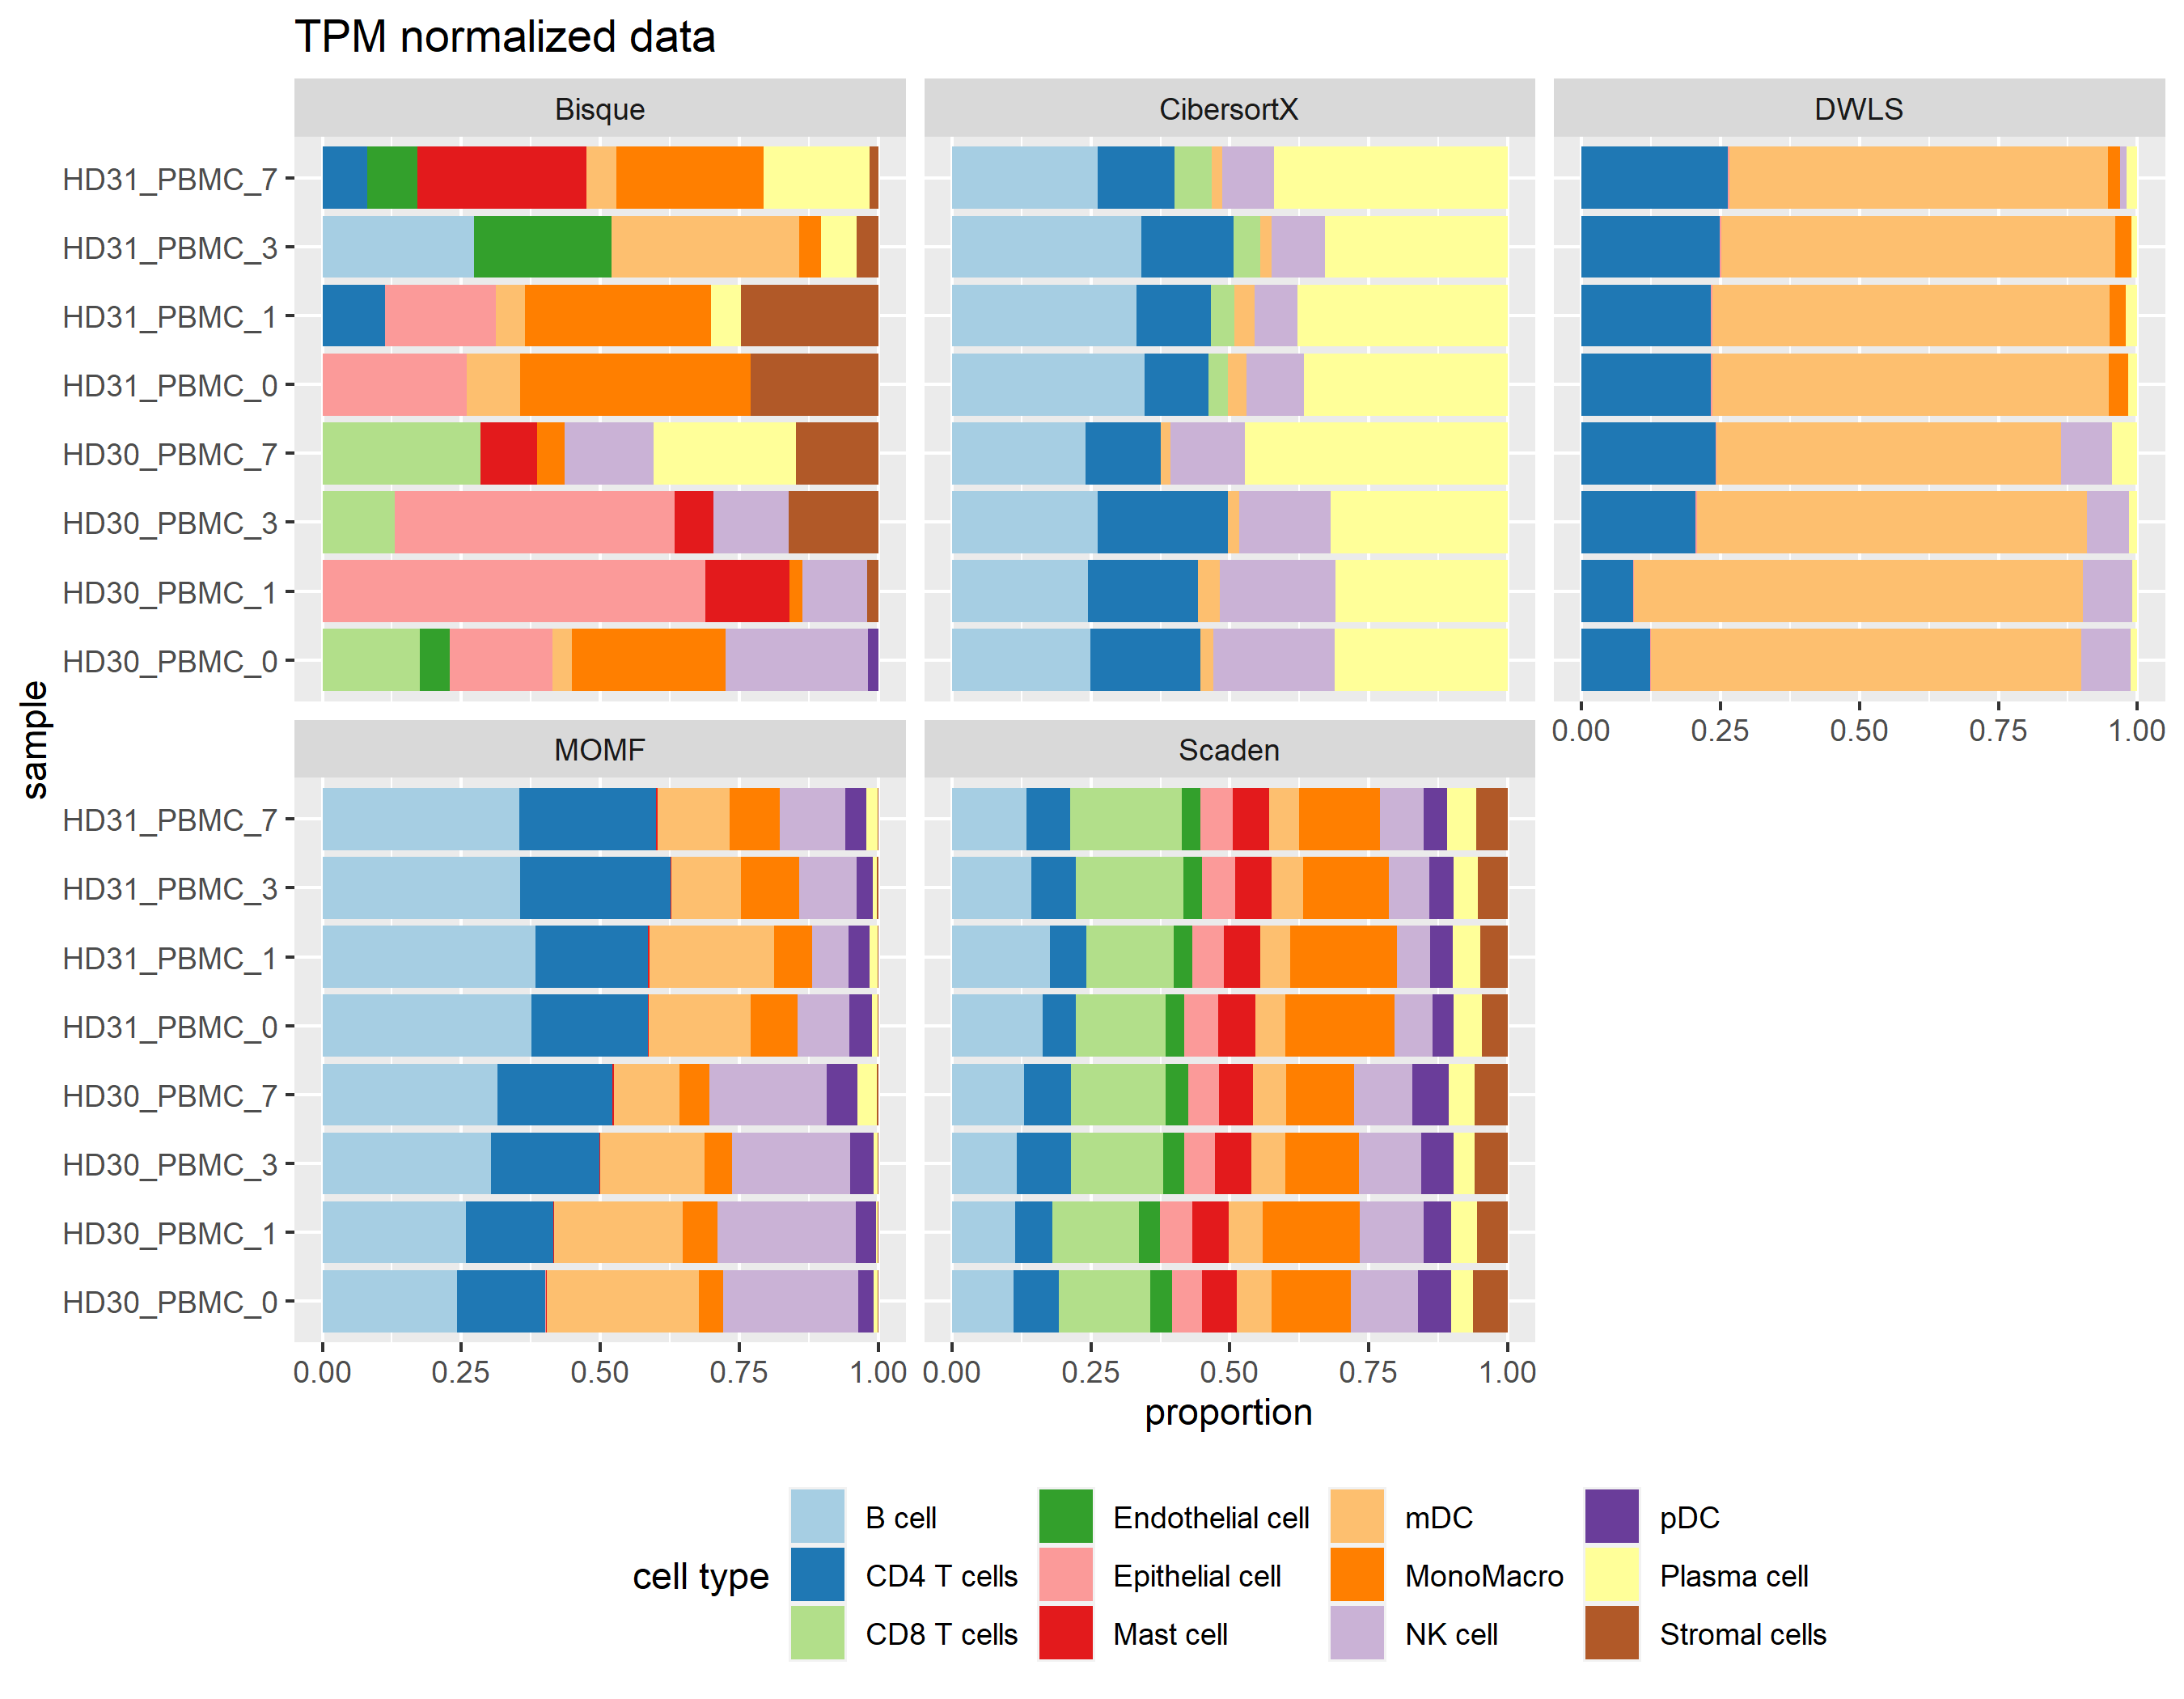
\includegraphics[width=0.8\linewidth]{images/propgrid_tpm}
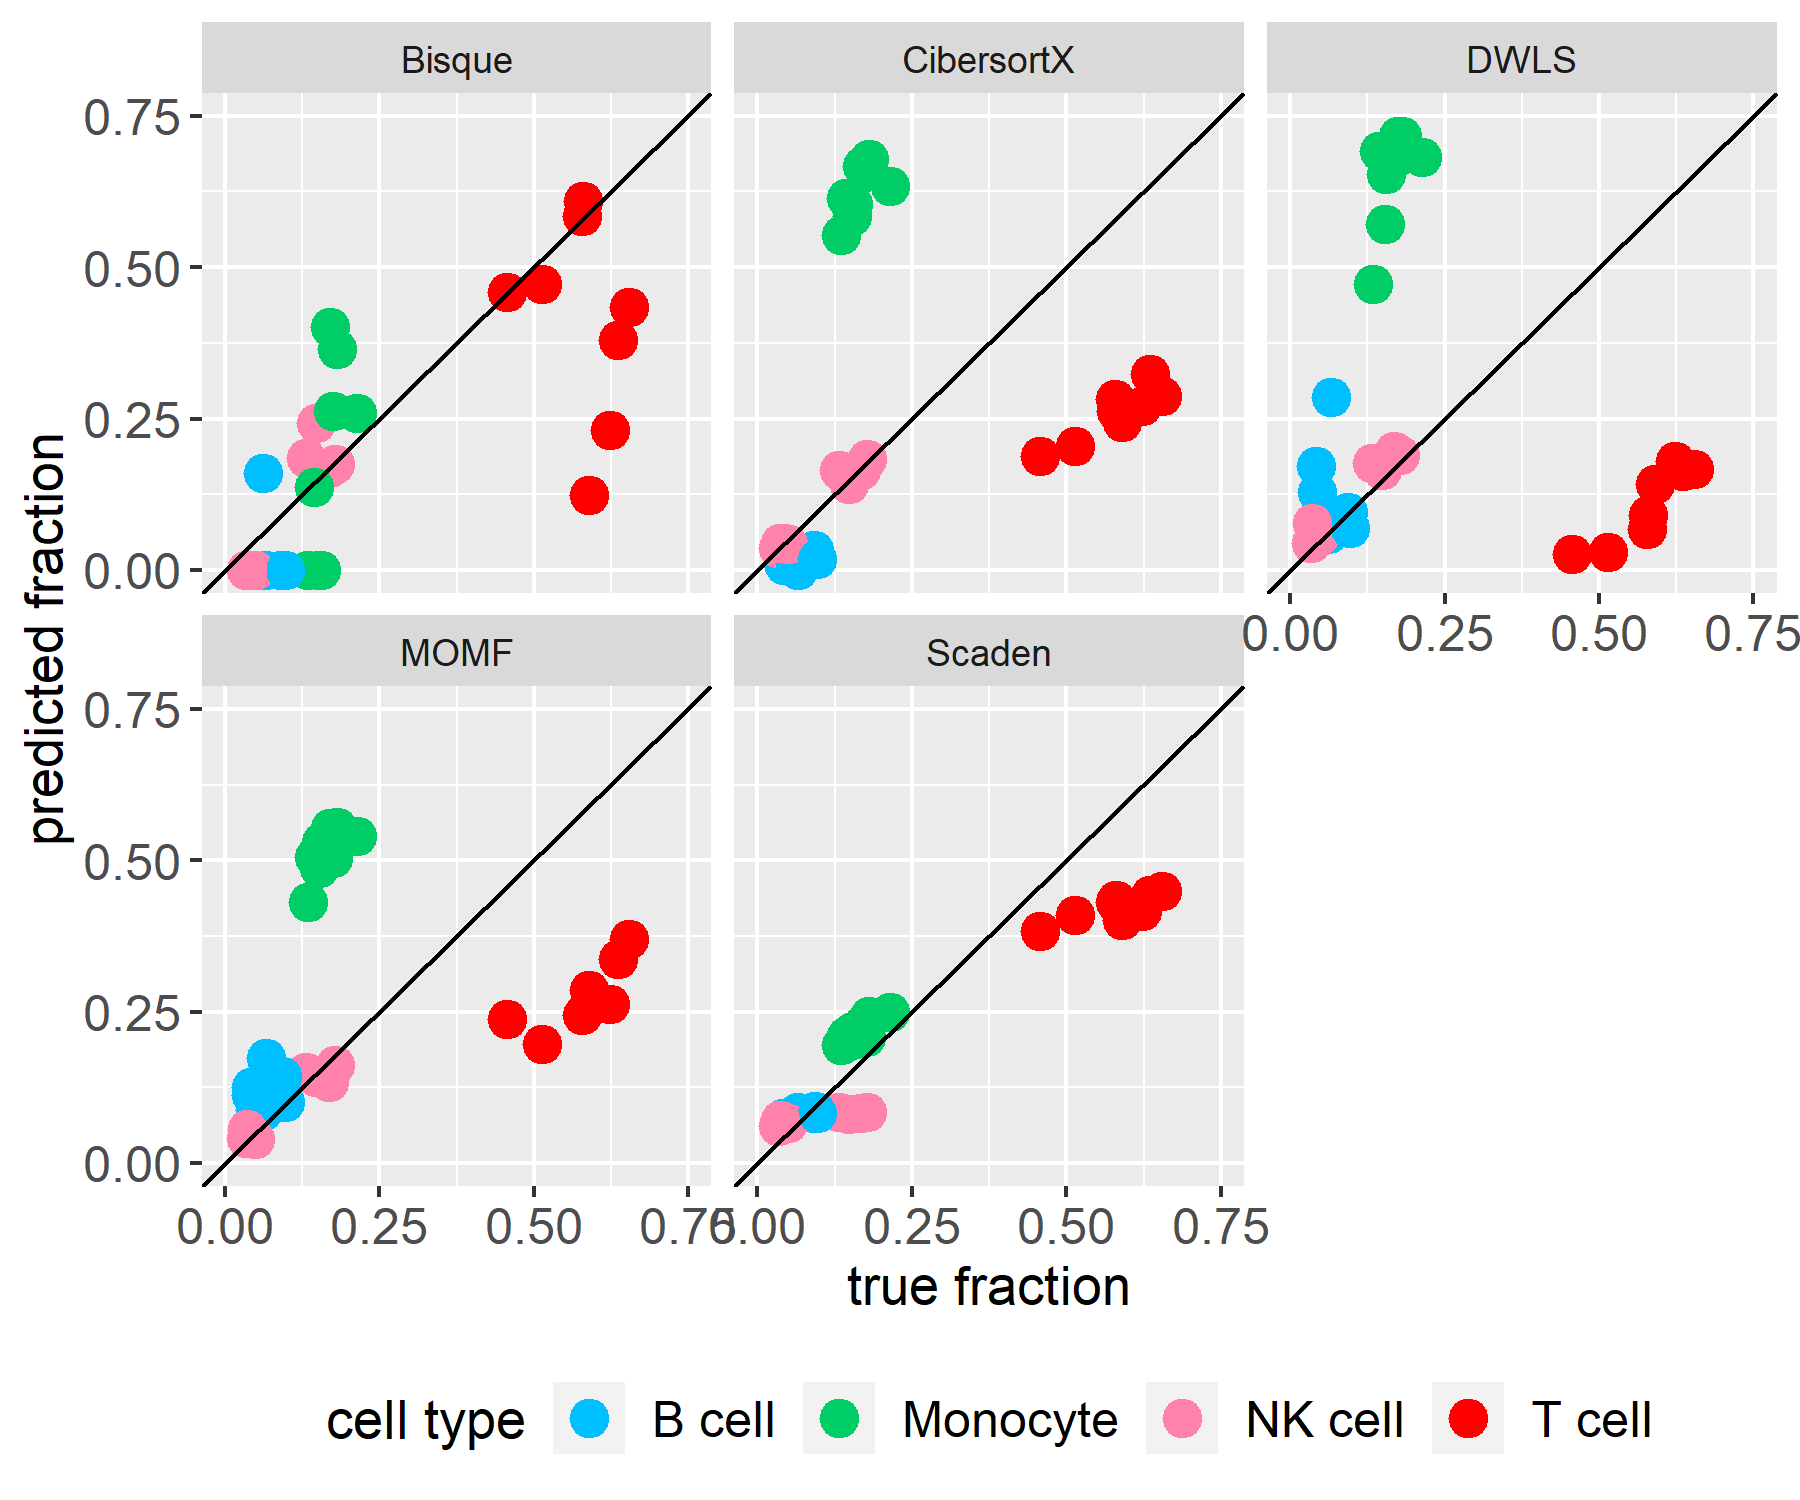
\includegraphics[width=0.8\linewidth]{images/predictionVsGroundtruth}

All in all, the methods differ a lot in their predictions. Bisque shows
very heterogenous results, which might be induced by its deconvolution
method. More details on that are provided a few figures below.
Predictions from Scaden, on the other hand, seem to be closest to the
ground truth, even though the prediction of the T cell fraction is way
off and also the dendritic cells are not that accurate. The results for
these two cell types are very interesting, as all methods calculate
their proportion wrong.

The inaccuracy of the prediction of T cells could be induced by TPM
normalization. To evaluate this theory, we analyzed the deconvolution
results for unnormalized single cell RNA-seq and bulk RNA-seq data as
well. The comparison of these predictions can be found in the figure
below.

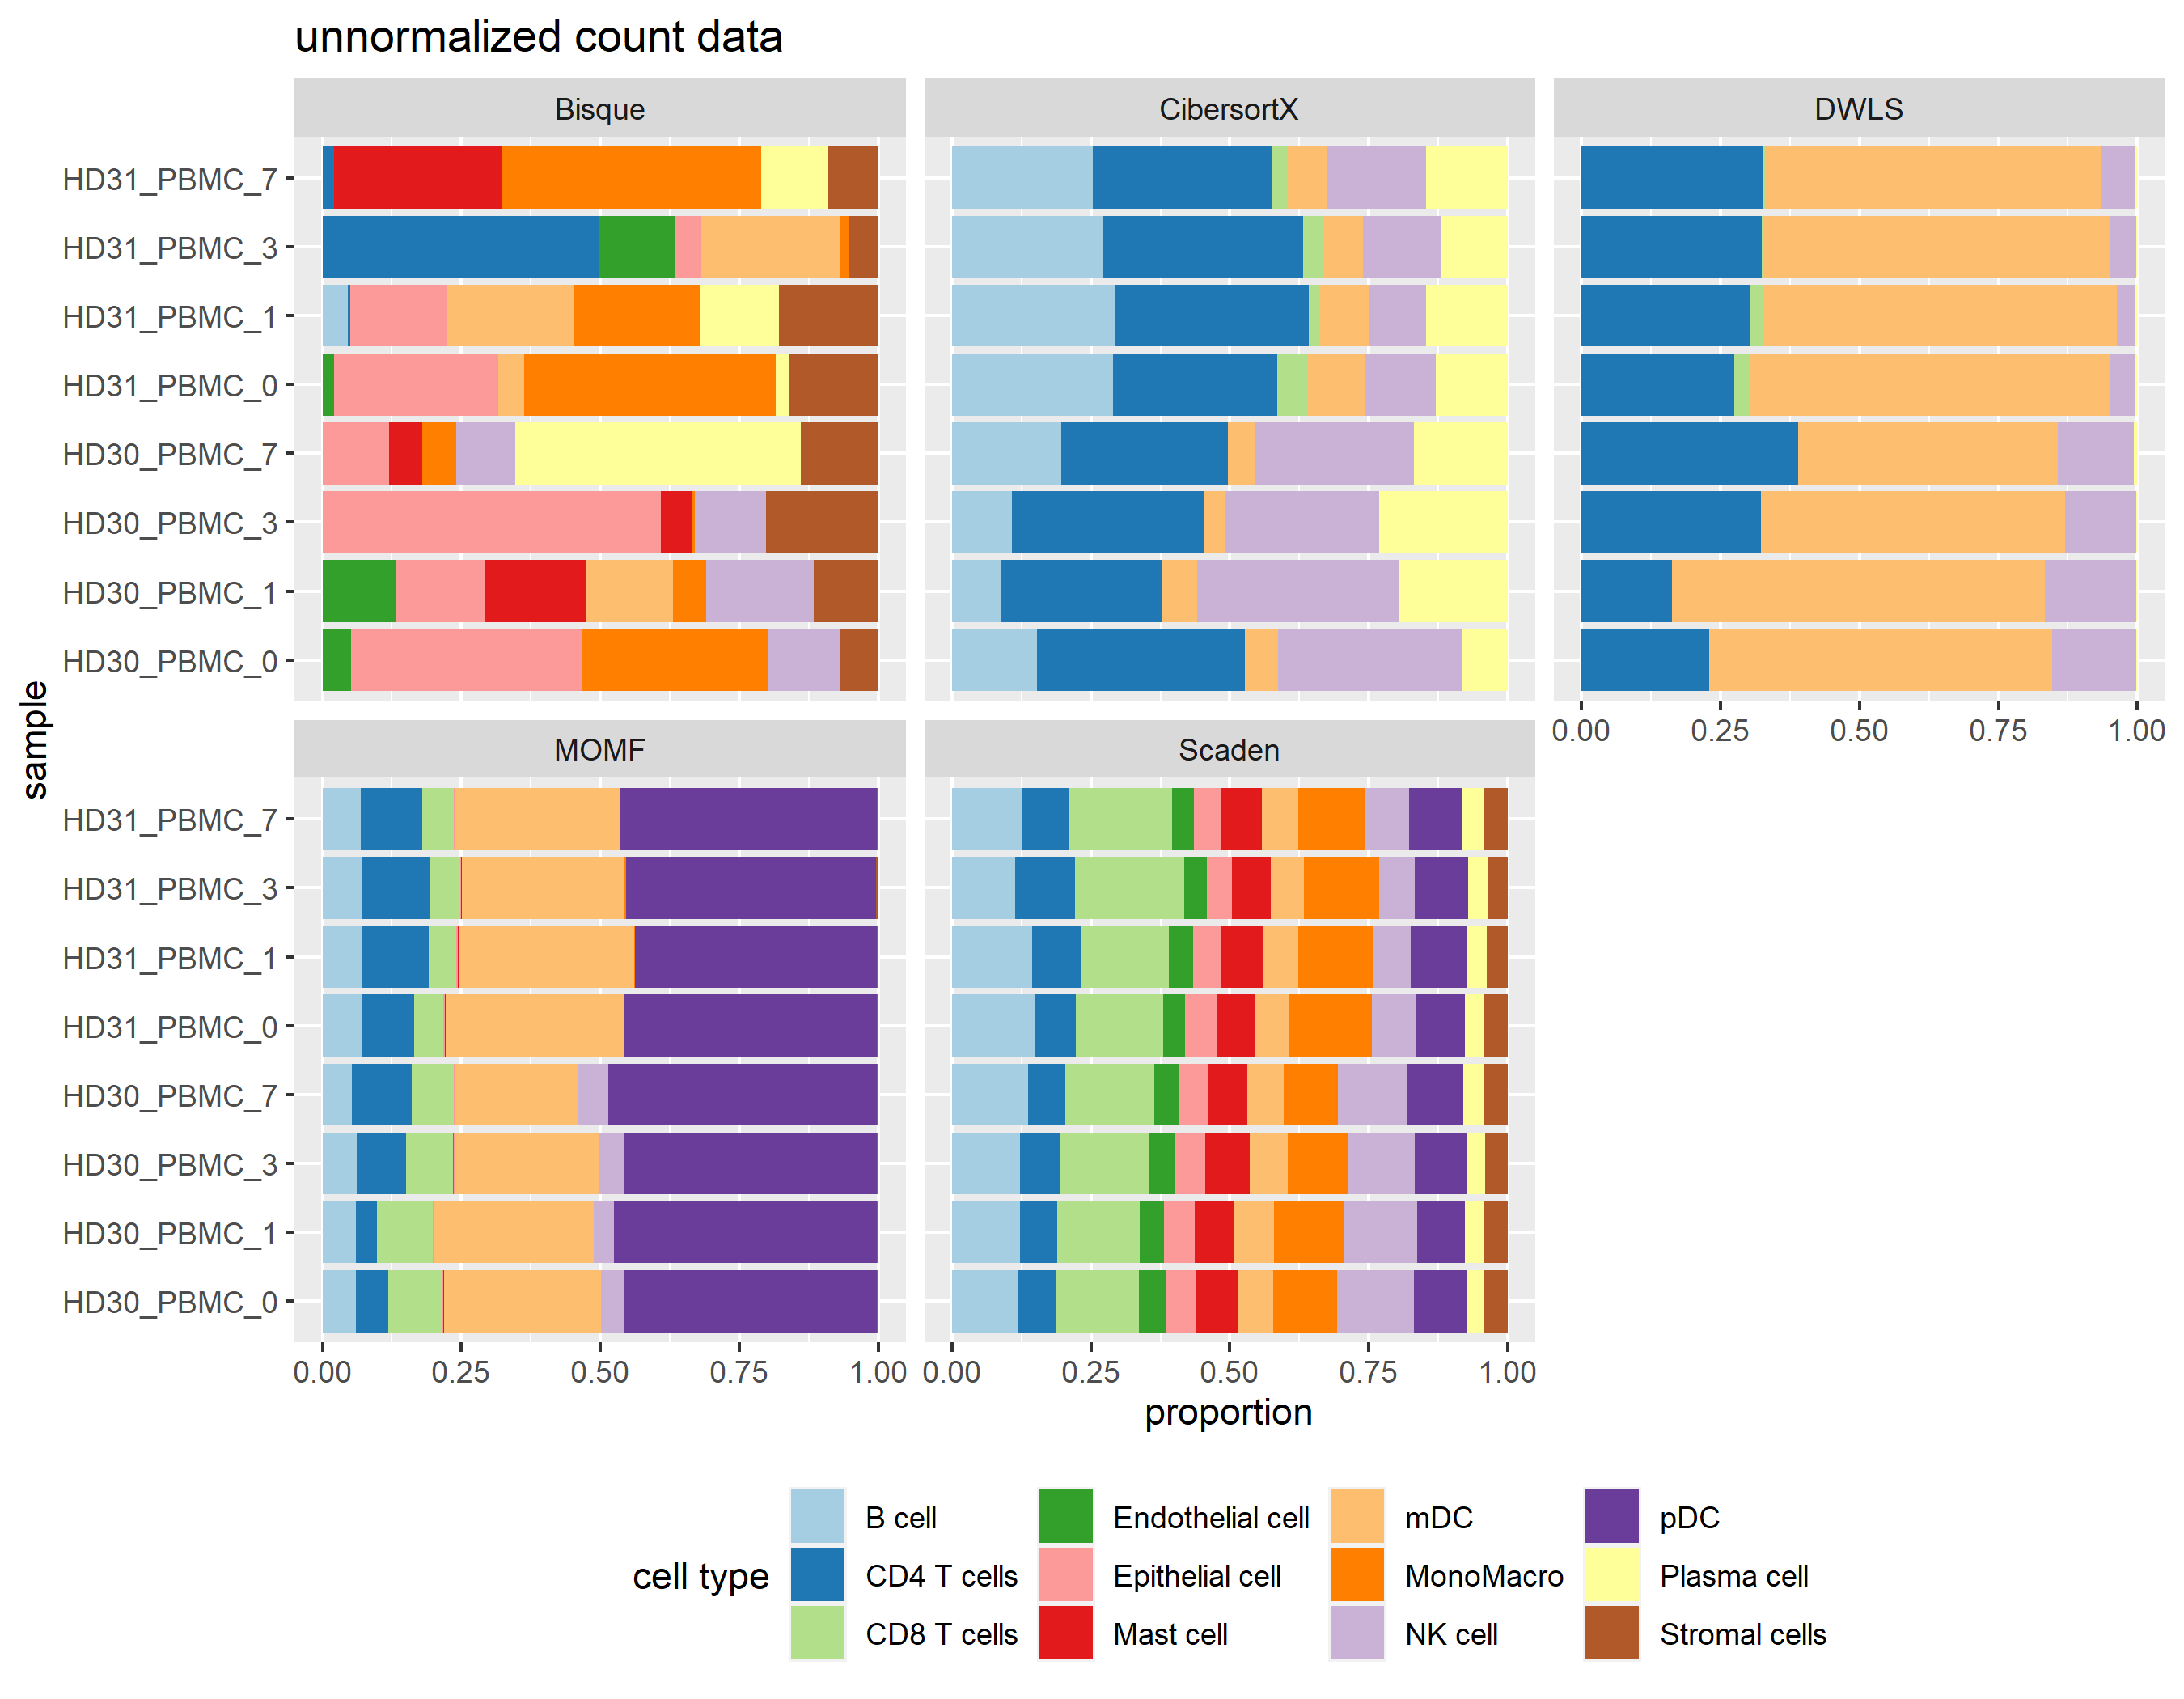
\includegraphics[width=0.8\linewidth]{images/propgrid_counts}
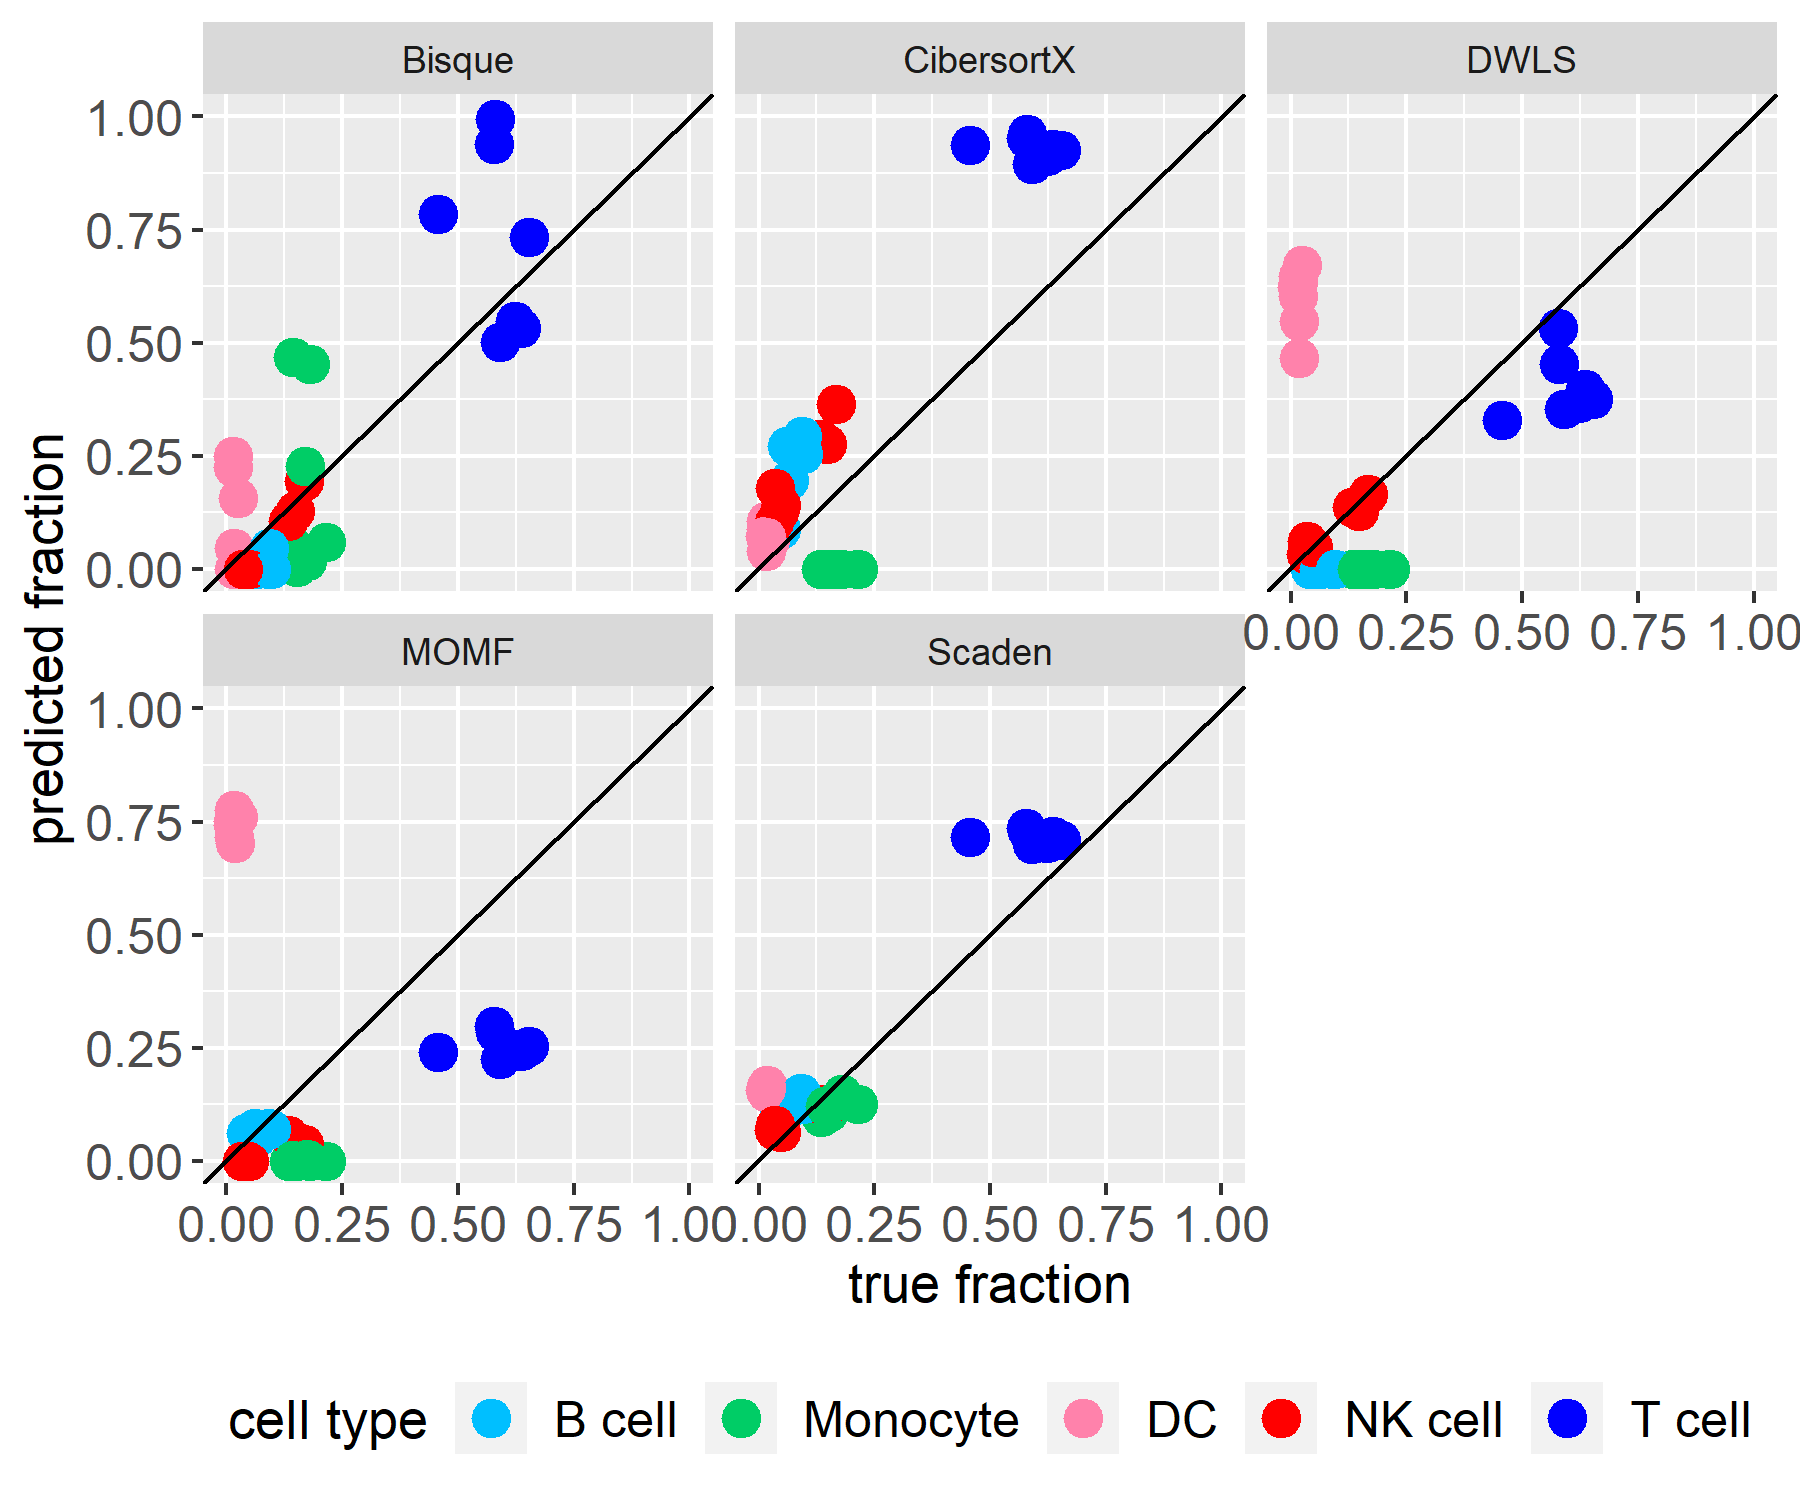
\includegraphics[width=0.8\linewidth]{images/predictionVsGroundtruth_unnormalized}

The predictions for the different cell type fractions still differ a lot
between the methods, as can be seen in the barplot. However, without TPM
normalization, the predictions for T cell fractions are slightly more
accurate. This is probably due to the fact that TPM normalization
removes the information about cell size and therefore how much mRNA is
present. As T cells account for the bigger cells in our immune system,
this ``counts per cell'' normalization method might not be a perfect fit
for immune deconvolution.

In contrast to the T cells, the predictions for dendritic cell fractions
are still very off. This phenomenon was already detected in the
benchmarking of first-generation immune deconvolution methods performed
by Sturm et al. (\protect\hyperlink{ref-Sturm2019}{Sturm 2019})

\hypertarget{comparison-with-first-generation-deconvolution-methods}{%
\subsection{Comparison with first-generation deconvolution
methods}\label{comparison-with-first-generation-deconvolution-methods}}

Another very important question is, how good the second-generation tools
are in comparison to the first-generation deconvolution methods. For
that purpose, we compared EPIC, quanTIseq, two first-generation methods
with their default parameters, with Scaden. We chose these methods,
since they showed a good performace in the benchmarking by Sturm et al.
(\protect\hyperlink{ref-Sturm2019}{Sturm 2019}). The deconvolution was
based on unnormalized data.

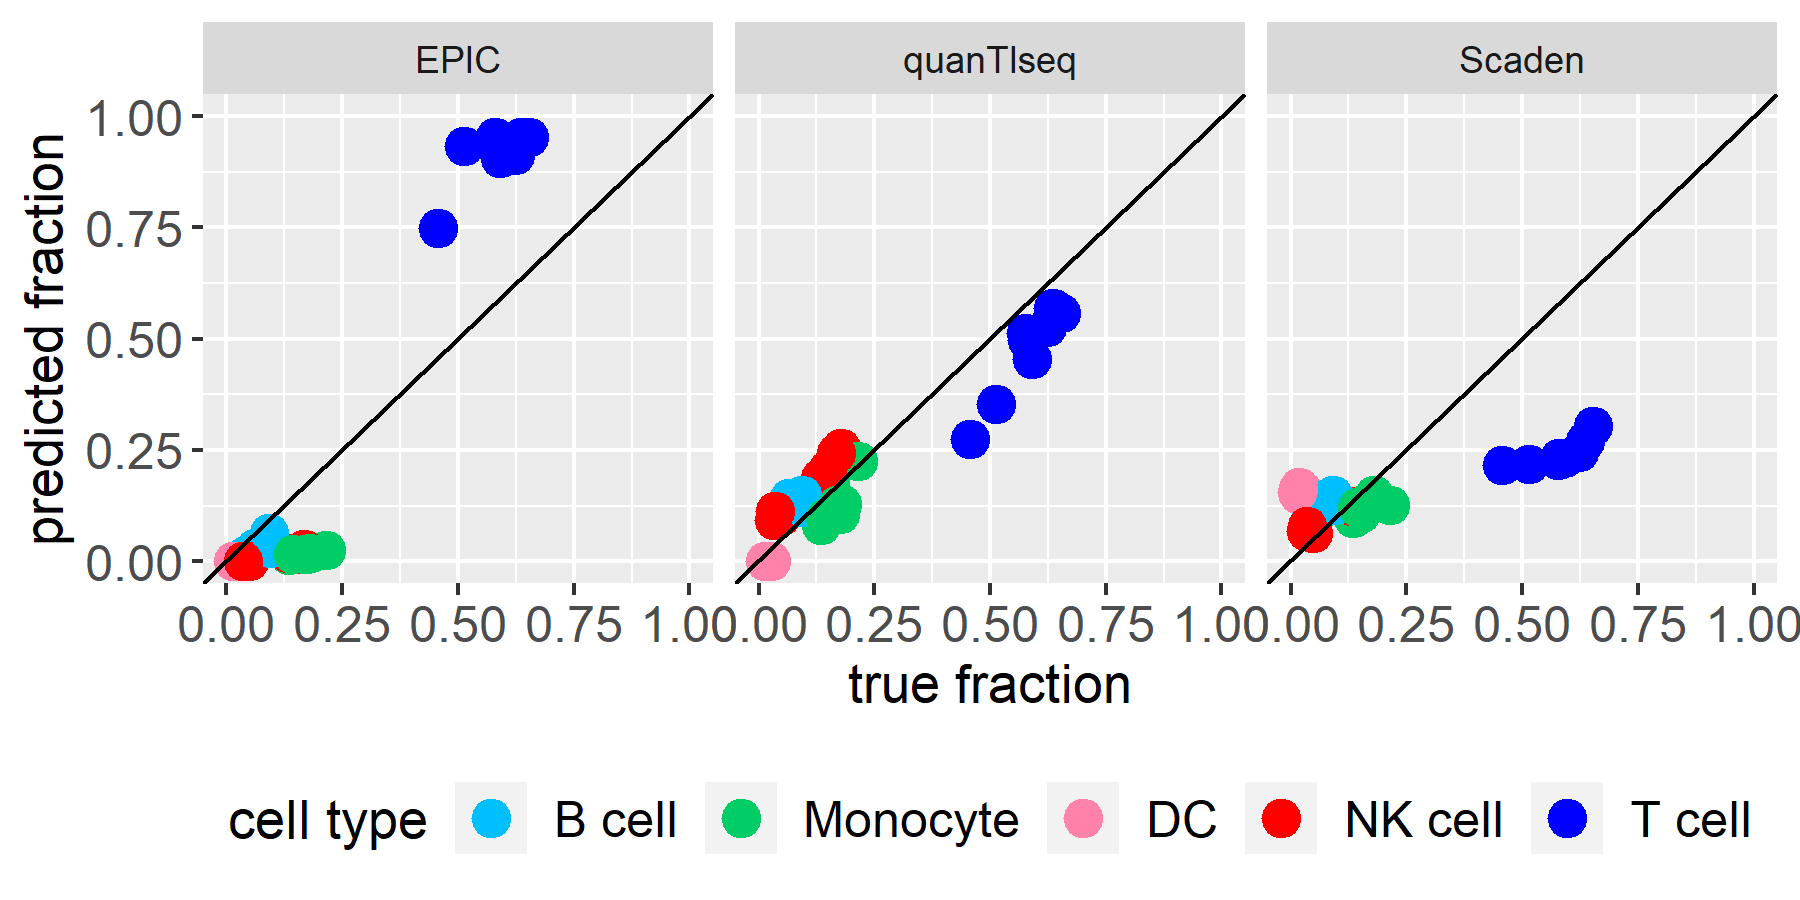
\includegraphics[width=0.8\linewidth]{images/predictionVsGroundtruth_unnormalized_firstGeneration}

As already addressed in section 1, first-generation deconvolution tools
use fixed, internal signature matrices containing only a limited set of
human cells. Second-generation tools bring more flexibility as they
allow the Derivation of cell-type specific signature matrices.

The advantage of fixed signature matrices is that they can be modulated
to fit to the bulk data very well. This is why quanTIseq and EPIC
produce very good predicitions in comparison to Scaden. However, other
datasets might not be suitable for these two methods. Furthermore,
Scaden does not fall behind regarding its precision, especially when
compared to EPIC.

However, this was just a small benchmark with one dataset. Different
datasets of different disease progressions and cell proportions might
show additional advantages or disadvantages of the methods. Generally it
can be said that second-generation tools provide other functionality and
thus make a good addition to the deconvolution package.

\hypertarget{signature-interchangeability}{%
\subsection{Signature
interchangeability}\label{signature-interchangeability}}

Since second-generation decovolution methods allow to derive
cell-type-specific expression signatures from single-cell RNA-seq
(scRNA-seq) as well as let the user provide their own signature matrix,
the possibility of interchanging signature matrices needs to be
examined.

Scaden is an exception as it does not produce a signature matrix but a
perceptron.

It is now possible to use every method which takes in a signature matrix
(everything except Scaden) with all other signature methods. This is
done by intersecting the genes of the bulk data, single cell data and
the signature matrix. In theory, this should not remove any data, as
most methods are unable to run with a different number of genes in the
signature matrix and the rest of the data. Nevertheless, this property
should be evaluated when the whole packages is benchmarked in detail.

\begin{longtable}[]{@{}llllll@{}}
\caption{Interchangeability table: `Yes' indicates, that a signature
matrix built by the method in the according column can be used for
deconvolution with the method from the according row.}\tabularnewline
\toprule
Deconv\_method & Bisque & CibersortX & DWLS & MOMF &
Scaden\tabularnewline
\midrule
\endfirsthead
\toprule
Deconv\_method & Bisque & CibersortX & DWLS & MOMF &
Scaden\tabularnewline
\midrule
\endhead
Bisque & yes & yes & yes & yes & -\tabularnewline
CibersortX & yes & yes & yes & yes & -\tabularnewline
DWLS & yes & yes & yes & yes & -\tabularnewline
MOMF & yes & yes & yes & yes & -\tabularnewline
Scaden & - & - & - & - & yes\tabularnewline
\bottomrule
\end{longtable}

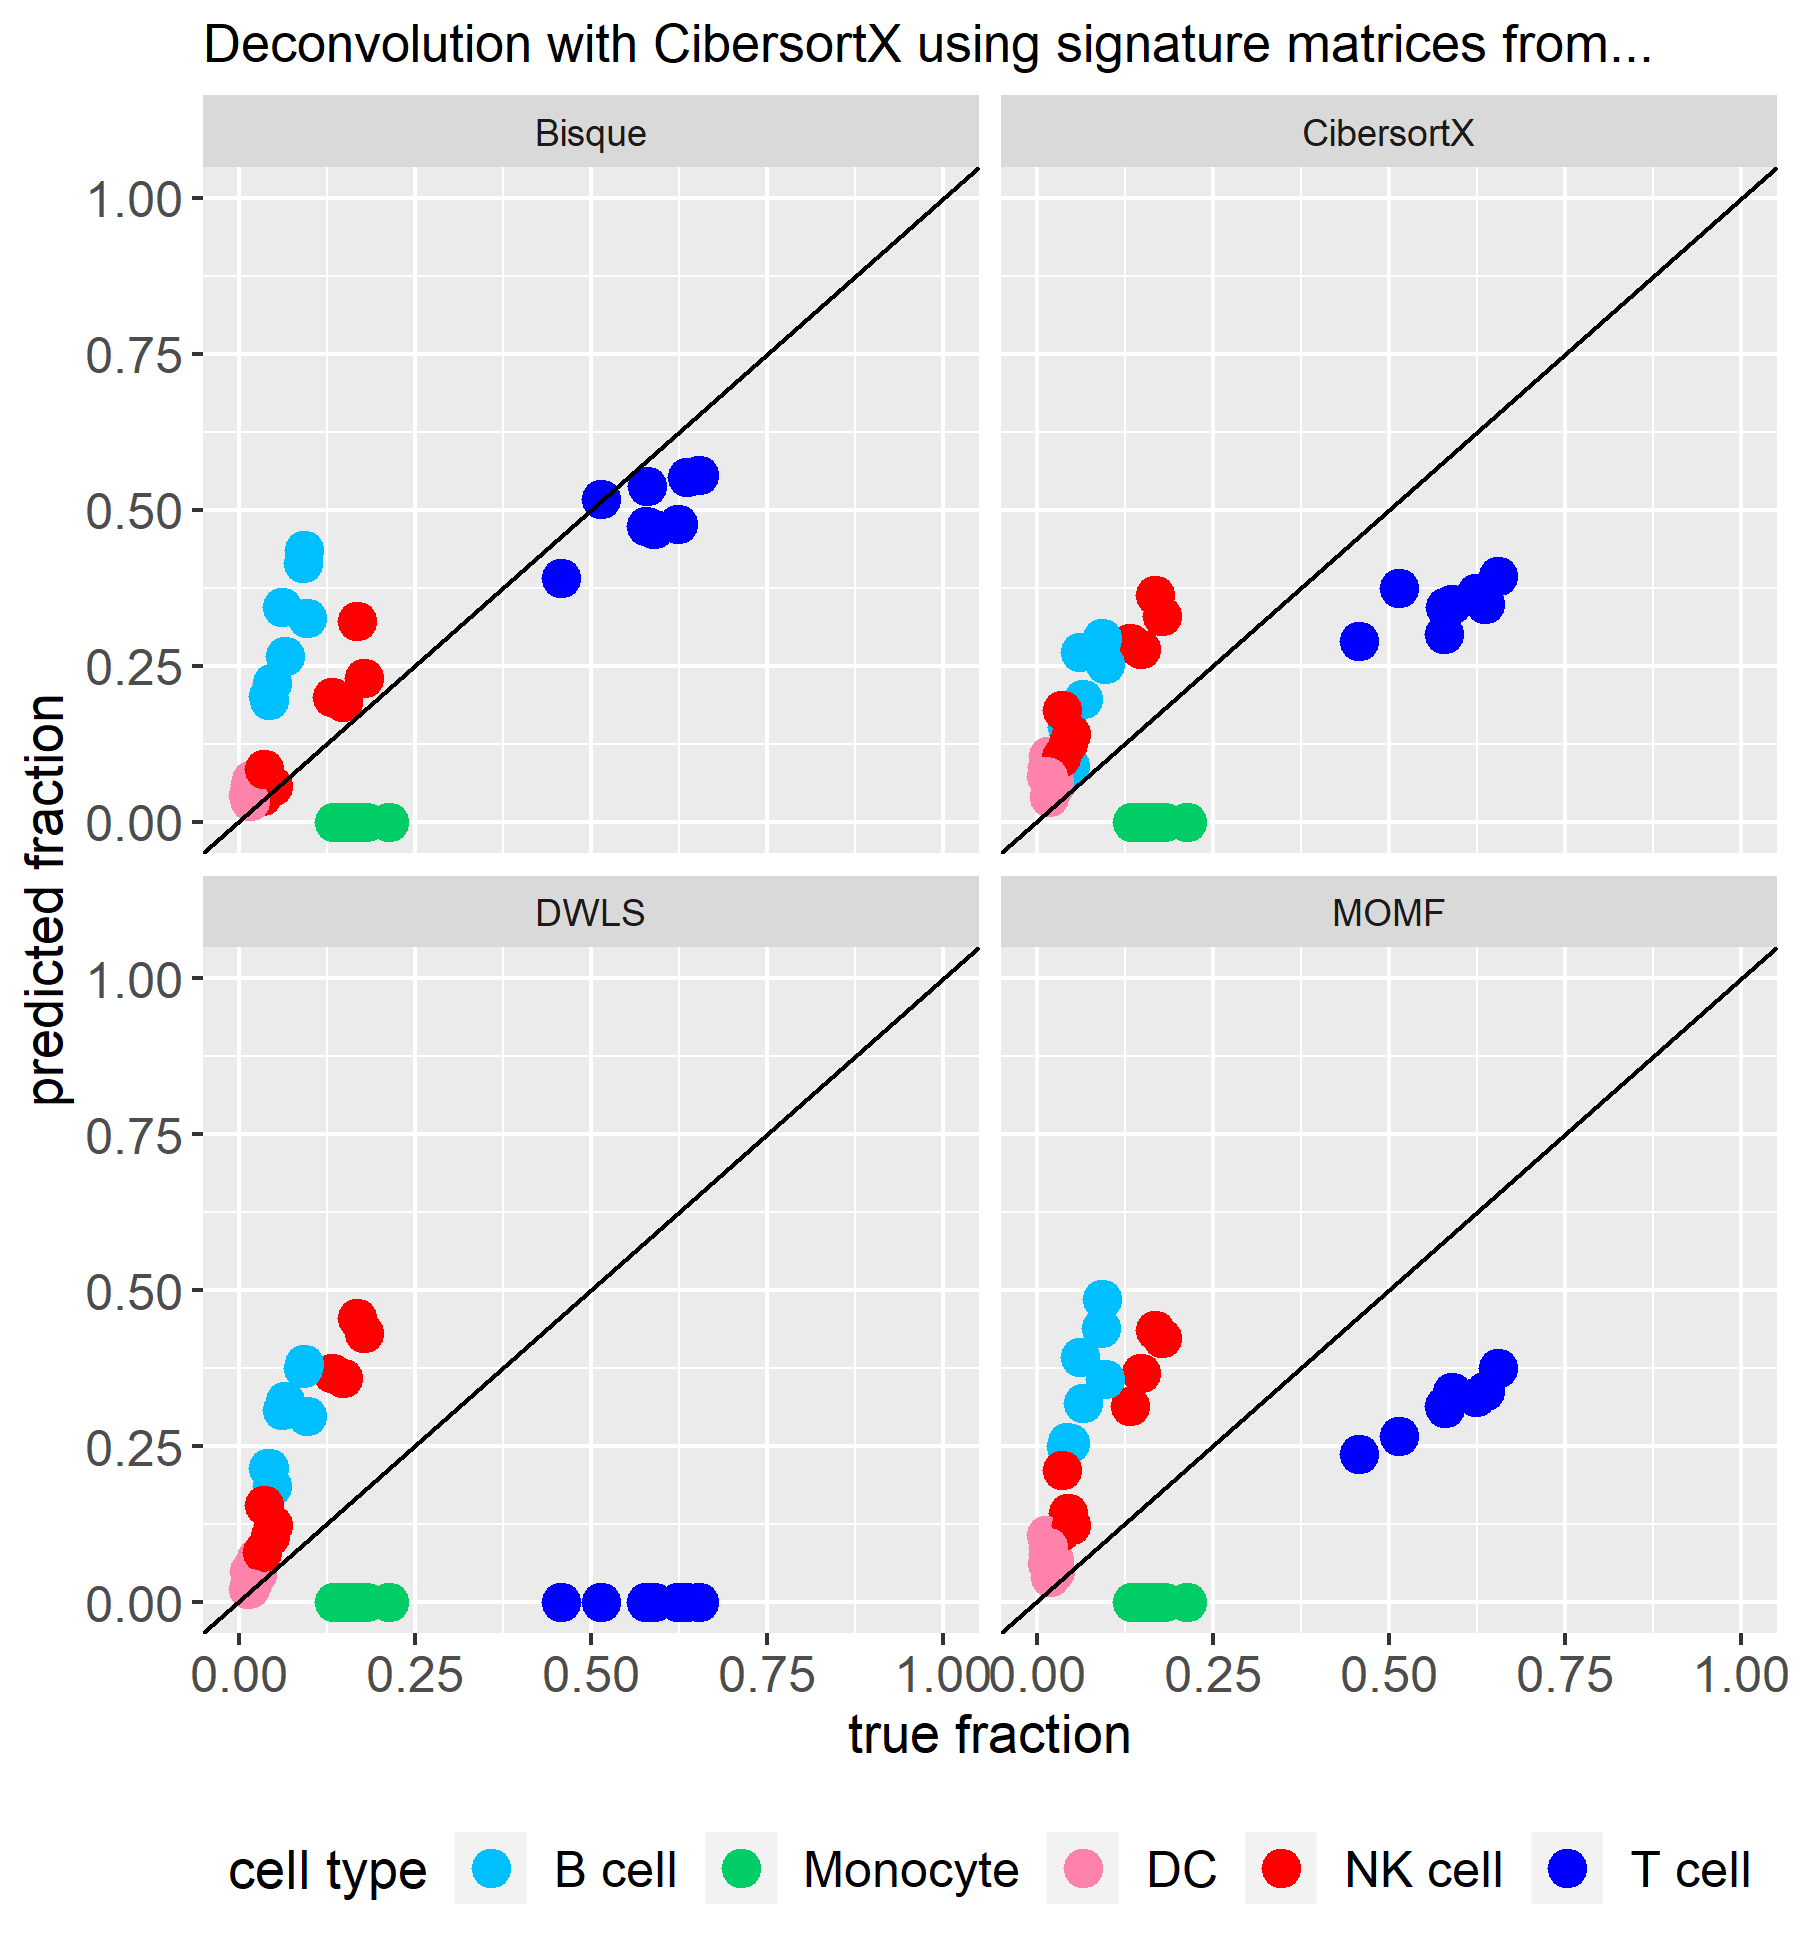
\includegraphics[width=0.45\linewidth]{images/ciber_matrices}
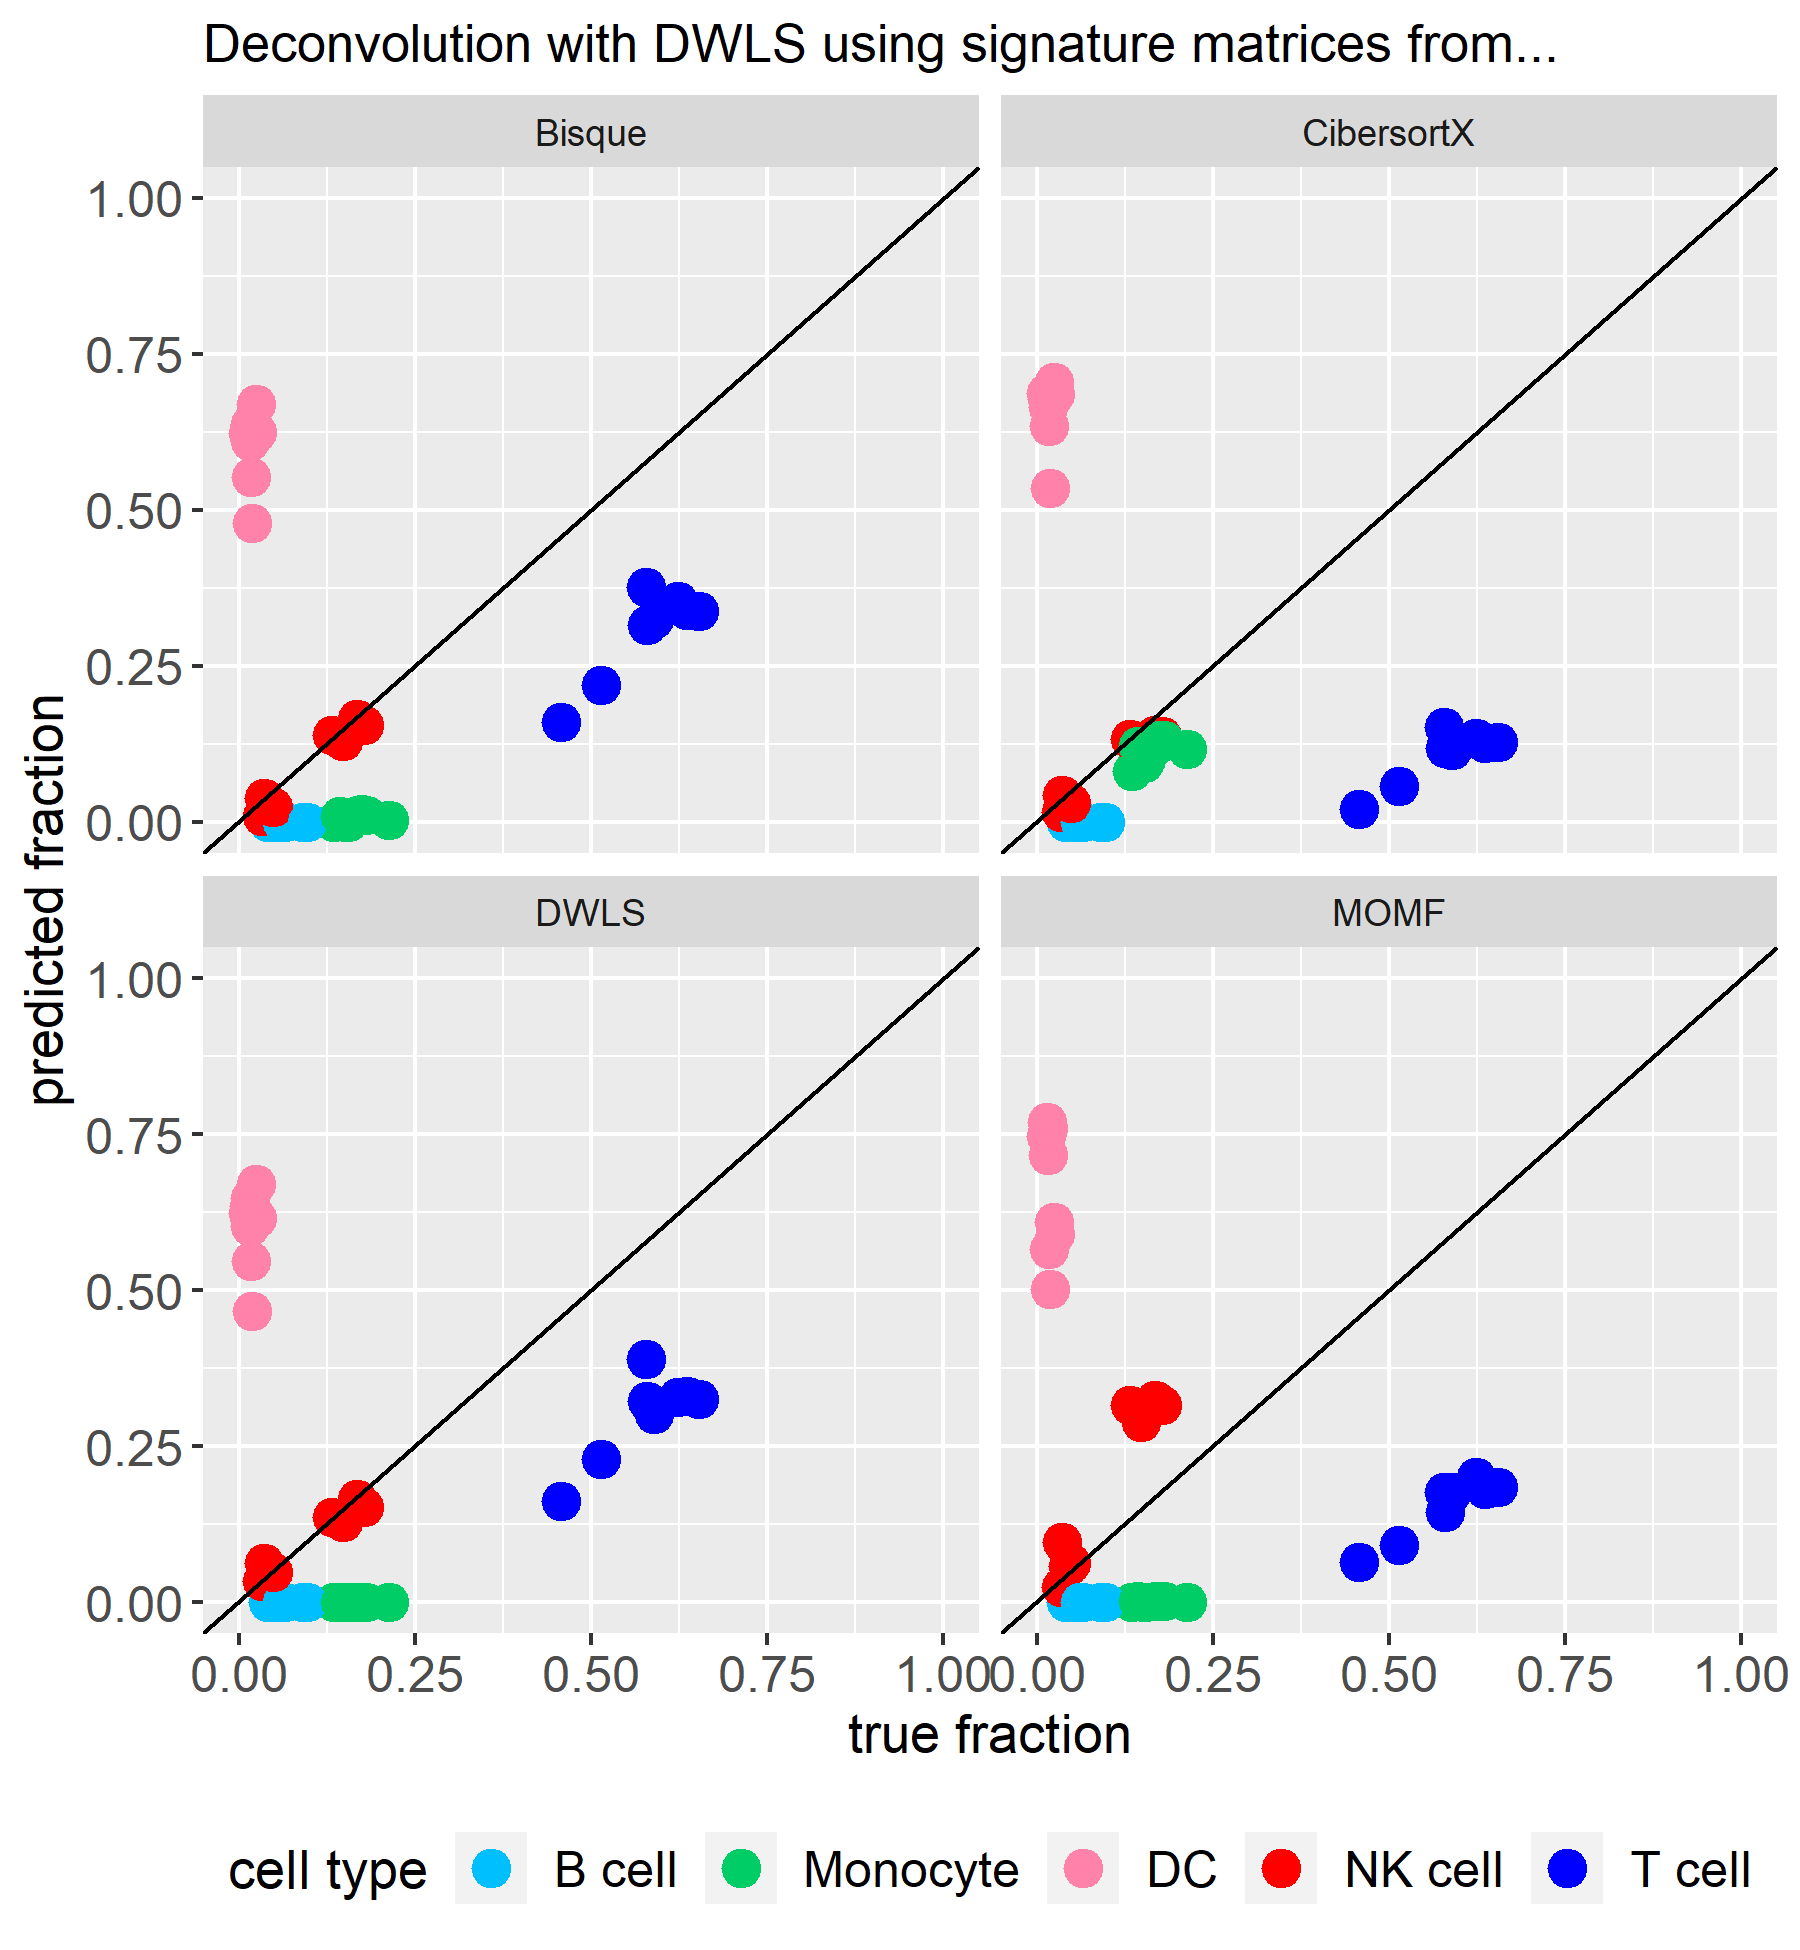
\includegraphics[width=0.45\linewidth]{images/dwls_matrices}
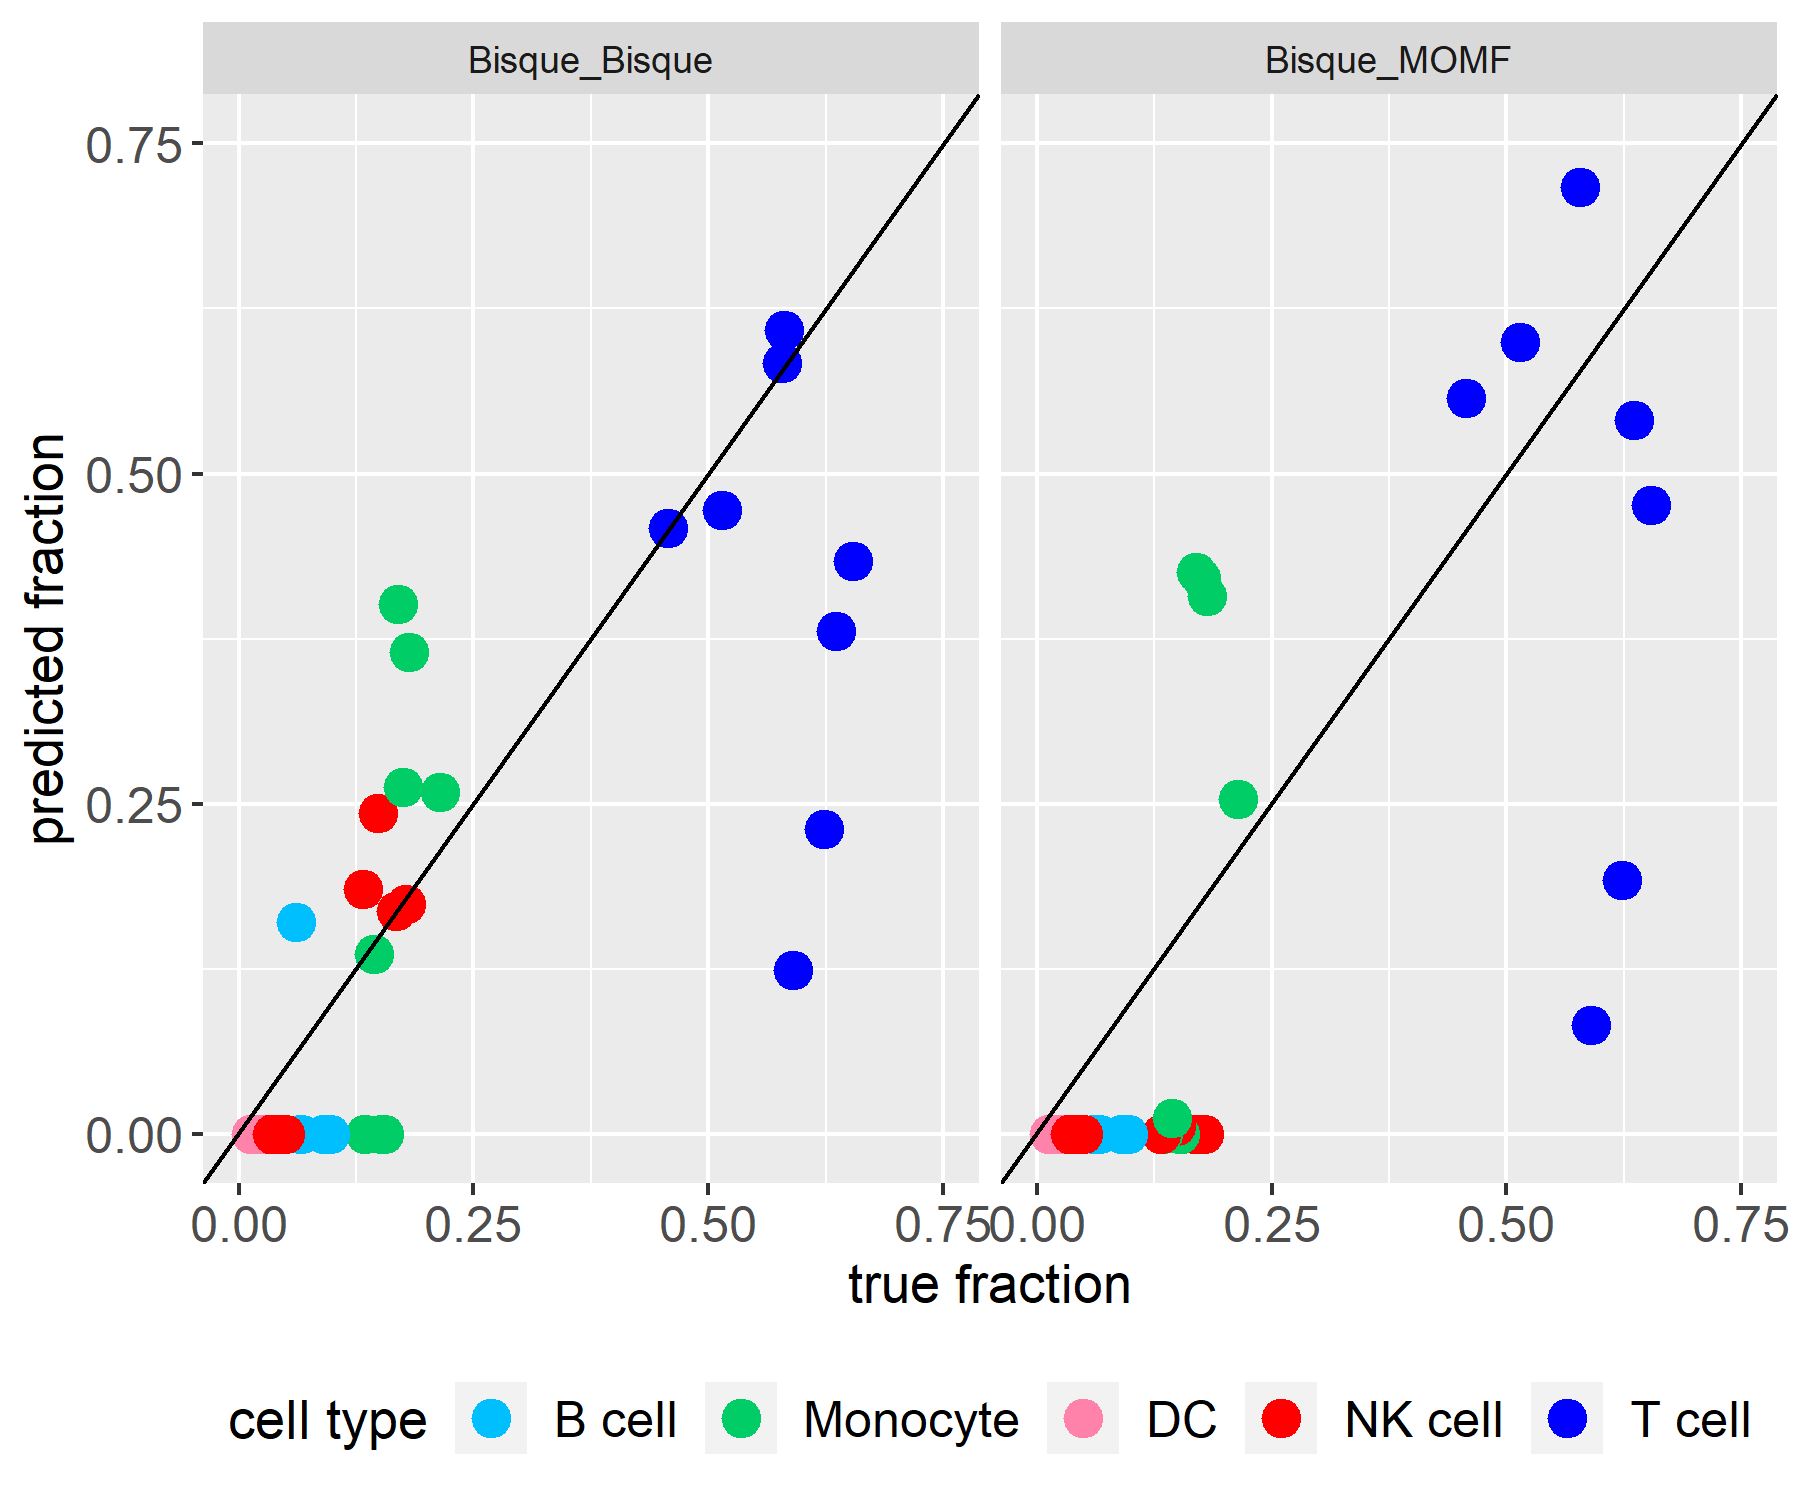
\includegraphics[width=0.45\linewidth]{images/bisque_matrices}
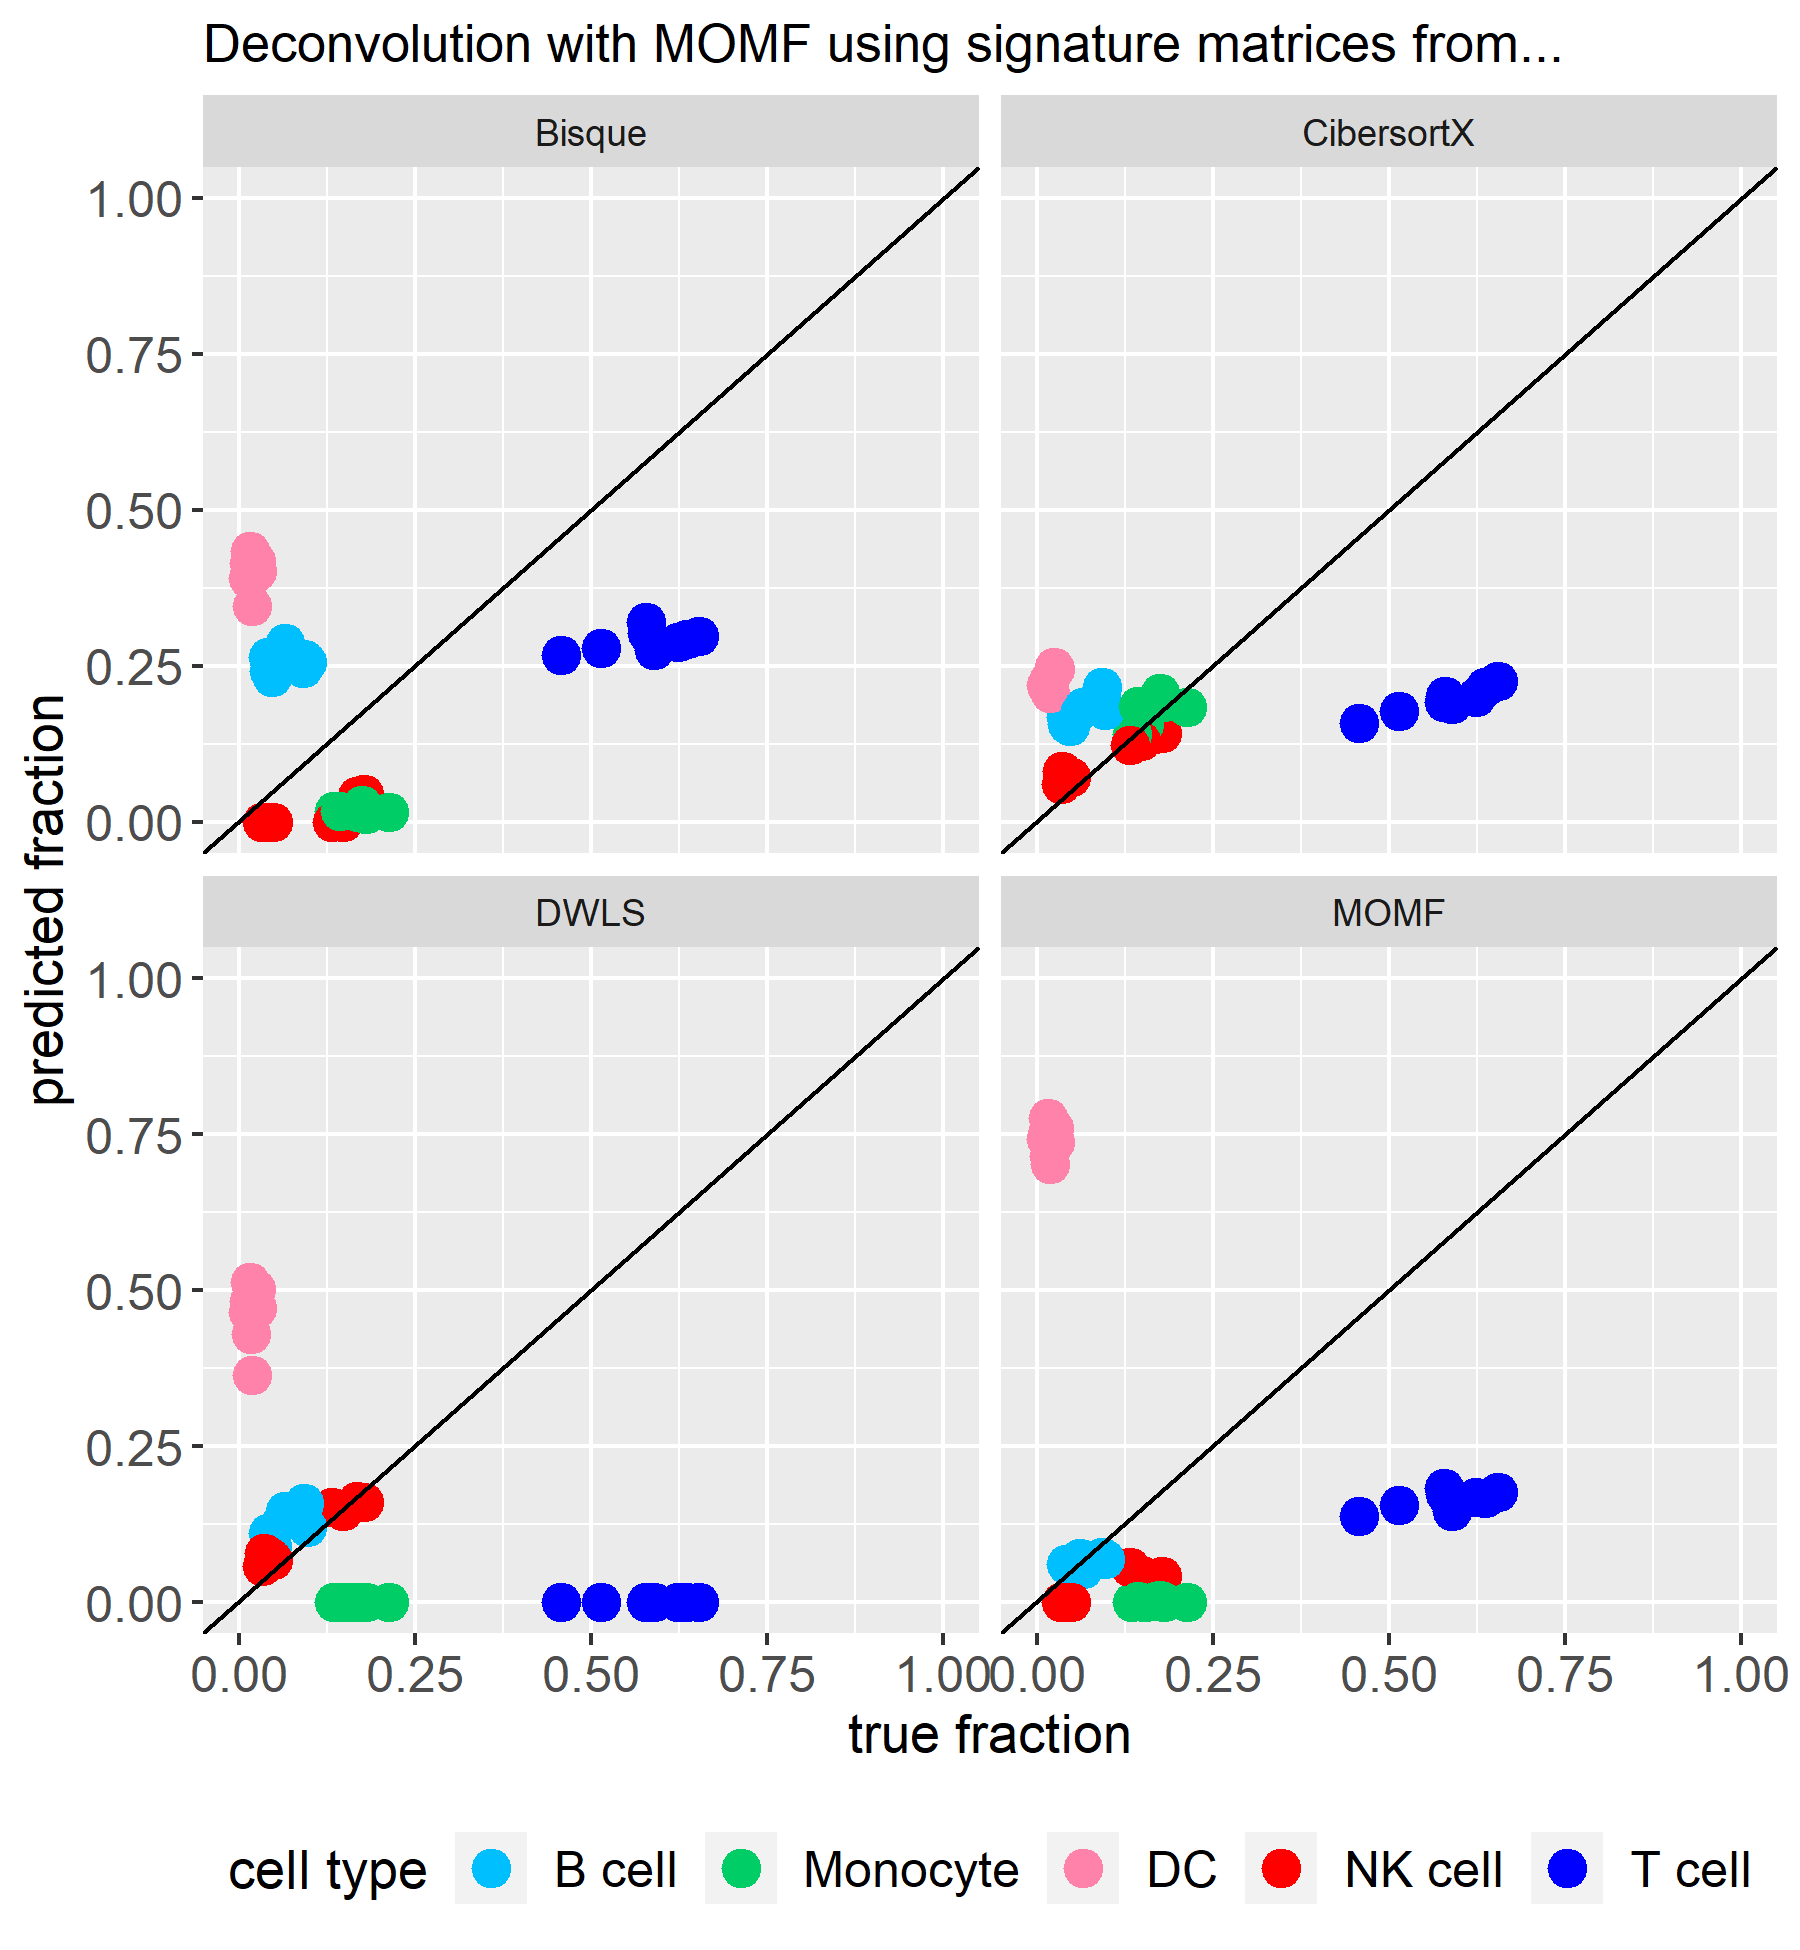
\includegraphics[width=0.45\linewidth]{images/momf_matrices}

As can be concluded from this figure, interchanging matrices between the
methods does not considerably improve the predictions. One might derive
small improvements especially when building the signature matrix with
Bisque or CibersortX, but the reason behind this needs further
examination in the future.

\hypertarget{distribution-of-work}{%
\section{5. Distribution of work}\label{distribution-of-work}}

We regularly met and were all involved in the general decision making
process. This list refers to who did the most work on those topics/who
was mainly responsible:

\begin{itemize}
\tightlist
\item
  Katharina: Implementation of MOMF, ReadMe, First edition of Vignette,
  Visualisation, Sample Data Sets, Benchmarking
\item
  Konstantin: Implementation of Bisque and CibersortX, Benchmarking,
  General Coordination and Planning
\item
  Nicolas: Implementation of Scaden, Unit tests, Data conversion methods
\item
  Yuyu: Implementation of DWLS, Continuous Integration, Documentation
  Website
\end{itemize}

\hypertarget{reference}{%
\section*{6. Reference}\label{reference}}
\addcontentsline{toc}{section}{6. Reference}

\hypertarget{refs}{}
\begin{CSLReferences}{1}{0}
\leavevmode\hypertarget{ref-Hoek2015}{}%
Hoek, Kristen et al. 2015. {``{A Cell-Based Systems Biology Assessment
of Human Blood to Monitor Immune Responses after Influenza
Vaccination}.''} \emph{PLOS One} 10.
https://doi.org/\url{https://doi.org/10.1371/journal.pone.0118528}.

\leavevmode\hypertarget{ref-Maynard2020}{}%
Maynard, Ashley et al. 2020. {``{Therapy-Induced Evolution of Human Lung
Cancer Revealed by Single-Cell RNA Sequencing}.''} \emph{Cell} 182.
https://doi.org/\url{https://doi.org/10.1016/j.cell.2020.07.017}.

\leavevmode\hypertarget{ref-Newman2015}{}%
Newman, Aaron M. et al. 2015. {``{Robust enumeration of cell subsets
from tissue expression profiles}.''} \emph{Nature Methods} 12.
\url{https://doi.org/10.1038/nmeth.3337}.

\leavevmode\hypertarget{ref-Sturm2019}{}%
Sturm, Gregor et al. 2019. {``{Comprehensive evaluation of
transcriptome-based cell-type quantification methods for
immuno-oncology}.''} \emph{Bioinformatics} 35.
\url{https://doi.org/10.1038/nrclinonc.2017.101}.

\end{CSLReferences}

\end{document}
